% Compile: pdflatex main; bibtex main; pdflatex main (twice).
\documentclass[11pt]{article}
\usepackage[letterpaper,margin=1in]{geometry}
\usepackage[T1]{fontenc}
\usepackage{lmodern,microtype}
\usepackage{amsmath,amssymb,amsthm,mathtools,bm}
\usepackage{booktabs,array,graphicx,enumitem}
\usepackage{xcolor}
\usepackage[numbers,sort&compress]{natbib}
\usepackage[colorlinks=true,linkcolor=blue!45!black,citecolor=blue!45!black,urlcolor=blue!45!black]{hyperref}
\usepackage{bookmark}
\hypersetup{pdftitle={Nearly Optimal Community Recovery by Spectral Likelihood Decoding},pdfauthor={Zhixin Zhou},pdfsubject={Spectral-only community recovery, end-to-end Chernoff-exponent guarantees, likelihood initialization and empirical evaluation}}
\setlength{\parskip}{3pt}
\setlist{nosep,leftmargin=*}
\newtheorem{theorem}{Theorem}[section]
\newtheorem{lemma}[theorem]{Lemma}
\newtheorem{proposition}[theorem]{Proposition}
\newtheorem{corollary}[theorem]{Corollary}
\theoremstyle{definition}
\newtheorem{definition}[theorem]{Definition}
\theoremstyle{remark}
\newtheorem{remark}[theorem]{Remark}
\newcommand{\Mis}{\operatorname{Mis}}
\newcommand{\E}{\mathbb E}
\newcommand{\PP}{\mathbb P}
\newcommand{\R}{\mathbb R}
\newcommand{\one}{\mathbf 1}
\newcommand{\diag}{\operatorname{diag}}
\newcommand{\col}{\operatorname{col}}
\newcommand{\rank}{\operatorname{rank}}
\newcommand{\tr}{\operatorname{tr}}
\newcommand{\norm}[1]{\lVert #1\rVert}
\newcommand{\abs}[1]{\lvert #1\rvert}
\newcommand{\argmax}{\operatorname*{arg\,max}}
\newcommand{\argmin}{\operatorname*{arg\,min}}
\numberwithin{equation}{section}
\title{Nearly Optimal Community Recovery by Spectral Likelihood Decoding}
\author{Zhixin Zhou}
\date{October 10, 2026\\\small Research manuscript}
\begin{document}
\maketitle
\begin{abstract}
We study community recovery using only the retained adjacency eigenpairs of a stochastic block model. For every fixed number of communities, we prove the expected misclassification bound $e^{-(1+o(1))I_n}$, where $I_n$ is the minimum exact Bernoulli Chernoff information. Writing $p=\max_{a,b}P_{ab}$, the model allows $p=\Omega(\log n/n)$ up to a fixed bound below one, with unequal community sizes and expected degrees. Its block probabilities are uniformly comparable and its block matrix satisfies a quantitative full-rank condition; no normalized matrix or community proportions are required to converge. The algorithm fits a complete Bernoulli working mixture to clipped spectral connection profiles. It starts with global-mean growing, repeatedly tests all single-component replacements using all-node likelihood gains, and accepts the greatest common working likelihood before a final EM update. A deterministic replacement lemma contracts population fitting loss by $1-1/K$ and, after empirical perturbation, proves weak recovery without an assumed initializer or convergence of each fit. Full-graph entrywise spectral bounds and a clipping-aware Chernoff argument then establish the leading oracle exponent, including at densities where inverse-polynomial confidence is insufficient. The proof concerns the stated repeated-replacement algorithm; growing alone is a separate procedure. We give a certified population failure of a finite-step growing path and evaluate the complete implementation on 60 graphs. These tests expose weak-signal failures and show no additional classification gain from replacement in that collection. Earlier 240-graph sparse-score experiments are retained with their original scope.
\end{abstract}
% ---- intro ----
\section{Introduction}\label{sec:introduction}

Community recovery in the stochastic block model (SBM) is a basic problem in network statistics. The model assigns each node to an unknown community and makes edge probabilities depend on the communities of their endpoints \cite{holland1983}. Two common approaches use different representations of the same data. Spectral methods reduce the adjacency matrix to a small number of eigenvectors and then cluster the embedded nodes. Likelihood methods compare how well alternative community assignments explain the observed connections. We show that likelihood-ratio information can be decoded from the retained spectrum to achieve nearly optimal community recovery for every fixed $K$ under uniform signal conditions and $p=\Omega(\log n/n)$, where $p=\max_{a,b}P_{ab}$, without returning to the original adjacency rows.

This question concerns the decoding rule as well as the embedding. A low-rank approximation is selected by a quadratic criterion, and standard spectral clustering applies a further Euclidean criterion through $K$-means. The oracle classifier for an SBM instead weights connections by logarithms of block probabilities and includes the contribution of absent edges. For a general connectivity matrix and unequal community sizes, its decision boundaries need not agree with nearest-center boundaries in the spectral embedding. Nevertheless, the fact that spectral reduction uses a quadratic objective does not itself imply that it discards the relevant likelihood information: a projection preserves every linear statistic whose weight vector belongs to the projected subspace.

\paragraph{Optimal recovery and likelihood refinement.}
The information-theoretic limits of the SBM are well developed. Abbe and Sandon \cite{abbe2015} characterize exact recovery in the general logarithmic-density SBM through Chernoff--Hellinger divergence and give efficient algorithms reaching that threshold. Zhou and Li \cite{zhouli2020} study the optimal error rate through Chernoff bounds and its application to community detection. We use these works to identify the oracle benchmark, while the statistical objective of the present paper is the leading-exponent form
\[
    \exp\{-(1+o(1))I\},
\]
where $I$ is the relevant pairwise Chernoff information. Throughout this paper, ``nearly optimal'' means attaining the leading oracle Chernoff exponent. We do not claim the refined multiplicative rate or a new global minimax lower bound.

Spectral initialization followed by likelihood refinement is also an established approach. Amini, Chen, Bickel and Levina \cite{amini2013} fit mixtures to blockwise connection counts using pseudo-likelihood and iterative updates. Gao, Ma, Zhang and Zhou \cite{gao2017} prove that a weakly consistent initializer followed by penalized local likelihood refinement achieves optimal misclassification performance under their assumptions. Zhou and Amini \cite{zhouamini2020} obtain optimal bipartite recovery using spectral initialization and pseudo-likelihood classification, and analyze a broader family of EM-type biclustering updates. A recent preprint of Wang \cite{wang2026vem} analyzes spectrally initialized variational EM in a general SBM, obtaining a leading Chernoff exponent while estimating parameters and reusing the original graph. In these methods the refinement uses information calculated from the original edge observations. Our algorithm imposes an additional restriction: once the selected adjacency eigenpairs have been computed, initialization, parameter updates, classification and component replacement use only those eigenpairs and quantities reconstructed from them.

\paragraph{Likelihood information in spectral representations.}
Spectral optimality is known in important special cases. Abbe, Fan, Wang and Zhong \cite{abbe2020} establish a first-order entrywise approximation for eigenvectors and show that, in the equal-sized symmetric two-community SBM at logarithmic density, an untrimmed spectral method attains the optimal recovery threshold and misclassification exponent. Their result already demonstrates that a spectral representation can retain the decisive local evidence. For homogeneous planted-partition SBMs with multiple, possibly unequal communities, Zhang \cite{zhang2024} gives matching error exponents for high-degree trimming followed by eigenvalue-weighted spectral clustering and $K$-means. His spectral exponent is distinguished from the information-theoretic exponent, so a sharp analysis of a spectral algorithm does not automatically establish its statistical optimality.

Probabilistic inference based on spectral embeddings predates the present work. Suwan et al.\ \cite{suwan2016} use Gaussian-mixture limits of adjacency spectral embedding to construct an empirical Bayes prior for block membership inference. This is a relevant example of using distributional information beyond Euclidean clustering; it does not establish a sparse large-deviation equivalence between our spectral scores and the oracle edge likelihood ratio. For lower densities, Zhou and Amini \cite{zhouamini2019} provide data-driven adjacency regularization and consistency analysis in the general bipartite setting. These consistency results do not by themselves prove preservation of the oracle error exponent.

\paragraph{Our approach.}
We retain the $K$ eigenpairs of the original adjacency matrix with largest absolute eigenvalues, including signal eigenvalues of either sign, and form clipped reconstructed connection profiles $q_i$. We compare profiles through the complete Bernoulli cross-entropy, including the nonedge term. A spectral estimate of the probability scale sets the logarithm floor. The resulting weighted-mean M-step has the same form at sparse and dense probabilities. Keeping the complete score is necessary for our density range: a dense two-community example in Section~\ref{sec:main-results} shows that the sparse score can lose a fixed fraction of the oracle exponent even when the parameters are known.

The growing initialization starts a component at the global profile mean, adds a node-profile candidate according to its likelihood gain over all nodes, and refits every component after each addition. Algorithm~1 then performs $\lceil\log n\rceil$ rounds of single-component replacement. In each round it tests every deletion position, chooses the best observed node candidate for that deletion by the same all-node gain, and fits the resulting profiles from uniform weights. The old fit and all trial endpoints compete under one working mixture likelihood. One final E-step and parameter M-step precede classification. This is an explicit repeated version of the existing replacement operation; it uses no randomized restart.

A short population argument is the key to the general-$K$ proof. Assign each of the $K$ true profiles to its nearest fitted profile. If a fitted profile is unused, it can be replaced without harming any assigned class. Otherwise the assignment is a bijection, and the fitted profile assigned to the class with largest loss can be replaced. In either case, inserting that true profile removes at least $1/K$ of the population hard loss. Every true community supplies a good observed candidate on the spectral approximation event. The exhaustive deletion scans therefore transfer this contraction to the empirical objective, up to vanishing relative error and the $n\log K$ cost of passing from hard to soft loss. Repetition makes the soft loss $o(n^2p)$, which certifies weak responsibilities simultaneously for all $K$ communities. This argument does not require the growing path to preserve a pure center at every intermediate stage or any EM fit to reach a global optimum.

The likelihood interpretation has a precise algebraic basis. If $\widehat\Pi$ is the retained empirical projector, the signed rank-$K$ reconstruction equals $A\widehat\Pi$. Under a population SBM projector, every block-constant Bernoulli contrast is preserved when $P$ has full rank. Empirical projection, clipping and parameter estimation introduce errors. We control them on a full-graph event whose failure probability is at most $C_H\exp(-Hnp)$ for every fixed $H$. This confidence level matters when the information scale exceeds $\log n$. First-order entrywise eigenspace analysis, a direct clipped Chernoff moment bound, and a deterministic invariant-basin argument handle the dependence of the fitted profiles on the same graph.

\paragraph{Contributions and scope.}
Theorem~\ref{thm:main-recovery} proves an end-to-end bound
\[
 \mathbb E\,\Mis(\widehat z,z)\le e^{-(1+o(1))I_n}
\]
for the complete deterministic algorithm and every fixed $K$. The assumptions are positive community proportions, comparable block probabilities, a uniform singular-value lower bound relative to $p$, probabilities bounded away from one, and $p=\Omega(\log n/n)$. Under comparability, this density condition implies expected degrees $\Omega(\log n)$. The assumptions allow heterogeneous degrees, intermediate densities and dense graphs, and neither $P/p$ nor the proportions need have limits. The theorem includes initialization and fitted parameters. It yields exact recovery when $\liminf I_n/\log n>1$ and concerns the leading oracle exponent, not a refined multiplicative rate.

The deterministic replacement theorem also identifies which algorithmic change closes the initialization gap. It applies to any starting fit in the observed profile box, including a poor growing endpoint. We do not claim a general-$K$ theorem for the unchanged growing-only algorithm. A certified five-community population example shows why a claim covering arbitrary finite intermediate EM budgets would fail: one update at each growing stage can leave a missing community and a duplicated center even at an arbitrarily large signal scale. One replacement round repairs that example; it does not establish failure of fully converged growing in general.

Finally, a reproducible 60-graph benchmark evaluates the complete Bernoulli implementation for $K=2,\ldots,6$ at logarithmic and dense probability scales, with the same reconstructed profiles used for sparse-score controls. Replacement does not change the classification error in this collection, and weak general signals remain difficult. The earlier paired 240-graph experiments are reported separately because they evaluate the historical sparse-score growing and repair procedures. These numerical results expose finite-sample behavior and implementation properties without substituting for the theorem.

Section~\ref{sec:algorithm} specifies the algorithm, Section~\ref{sec:main-results} states the recovery results, and Section~\ref{sec:experiments} reports experiments. Proofs are in the appendix.

% ---- algorithm ----
\section{Spectral likelihood decoding}
\label{sec:algorithm}

\subsection{Model and retained information}
Let $A$ be the adjacency matrix of an undirected graph without self-loops. Conditional on $z\in[K]^n$, the upper-triangular entries are independent, with
\begin{equation}
 A_{ij}\sim\operatorname{Bernoulli}(P_{z_i z_j}),\quad i<j,
 \qquad A_{ji}=A_{ij},\quad A_{ii}=0.
 \label{eq:sbm}
\end{equation}
We follow Zhou and Li~\citep{zhouli2020}: $P$ is the symmetric block probability matrix, $p_{aj}=P_{a,z_j}$, and $p_{a*}$ is the connection profile of community $a$. Write $Z_{ia}=\one\{z_i=a\}$, $n_a=\sum_iZ_{ia}$, $\pi_{a,n}=n_a/n$, and
\[
 p=\max_{a,b}P_{ab}.
\]
The known community number $K\ge2$ is any fixed integer. Our uniform model and density conditions are, for fixed positive constants $\pi_0,\kappa,\eta$,
\begin{align}
 n_a&\ge\pi_0n,\qquad P_{ab}\ge\kappa p\quad(a,b\in[K]),\qquad
 \sigma_{\min}(P)\ge\kappa p,
 \label{eq:model-conditions}\\
 p&\le1-\eta,\qquad p=\Omega(\log n/n).
 \label{eq:density-condition}
\end{align}
We may take $\kappa\le1$. Neither $P/p$ nor the community proportions need converge. The probability matrix may vary with $n$ within these bounds. In particular, there is no requirement that $(n/\log n)P$ be fixed.

For $z_i=a$, the expected degree is
\begin{equation}
 \E[\deg(i)\mid z]
   =\sum_b(n_b-\one\{a=b\})P_{ab}.
 \label{eq:expected-degree}
\end{equation}
These expectations lie between $\kappa(n-1)p$ and $np$ and may differ across communities. Thus they are uniformly of order $np$, and \eqref{eq:density-condition} implies that all expected degrees are $\Omega(\log n)$. The density condition permits intermediate densities and constant edge probabilities. The probability-comparability and singular-value conditions ensure a uniformly separated, well-conditioned signal; degree alone does not imply identifiability.

Retain the $K$ eigenpairs of the original adjacency matrix with largest absolute eigenvalues:
\begin{equation}
 AU=U\Lambda,\qquad U^\top U=I_K,\qquad
 \widetilde A=U\Lambda U^\top.
 \label{eq:representation}
\end{equation}
Both signs of signal eigenvalues are allowed. Every subsequent operation uses only $(U,\Lambda)$, including initialization, fitting, replacement and classification.

\subsection{Why spectral information can retain a likelihood ratio}
For testing $z_i=a$ against $z_i=b$ with the other labels and $P$ known, put
\begin{equation}
 w_j^{ab}=\log\frac{p_{aj}(1-p_{bj})}{p_{bj}(1-p_{aj})},\qquad
 c_i^{ab}=\sum_{j\ne i}\log\frac{1-p_{aj}}{1-p_{bj}}.
 \label{eq:oracle-contrast}
\end{equation}
The exact incident-edge Bernoulli LLR is $L_i^{ab}=A_iw^{ab}+c_i^{ab}$. Extending $w_i^{ab}$ by the same block formula does not change it because $A_{ii}=0$. The contrast vector is block constant.

\begin{proposition}[Preservation of likelihood contrasts]
\label{prop:exact-preservation}
With $\Pi=UU^\top$, the identity
\begin{equation}
 \widetilde A=A\Pi,\qquad
 \widetilde A_iw-A_iw=A_i(\Pi-\mathrm{Id})w
 \label{eq:projection-identity}
\end{equation}
holds for every vector $w$. If $w\in\operatorname{col}(U)$, the corresponding linear statistic is preserved exactly. If $P$ is nonsingular, then $\operatorname{col}(ZPZ^\top)=\operatorname{col}(Z)$, which contains every $w^{ab}$.
\end{proposition}

The first identity follows from the eigenvector equation. For the second assertion, use the factorization
$ZPZ^\top=(ZN^{-1/2})(N^{1/2}PN^{1/2})(ZN^{-1/2})^\top$, where $N=Z^\top Z$. Thus the spectral decomposition retains directions on which the likelihood acts; it need not itself optimize a likelihood. The actual mean is
\begin{equation}
 \E[A\mid z]=ZPZ^\top-\operatorname{diag}(P_{z_i z_i}).
 \label{eq:mean}
\end{equation}
The statistical analysis below accounts for this diagonal correction and for the difference between the empirical and population subspaces.

\subsection{Observed profiles and the complete Bernoulli score}
To define logarithms of reconstructed probabilities, set
\begin{equation}
 s=\max\{1,\|\Lambda\|_{\mathrm{op}}\},\qquad
 \varepsilon_n=c_0s/n,\qquad
 q_{ij}=\operatorname{clip}(\widetilde A_{ij},\varepsilon_n,1-\varepsilon_n),
 \label{eq:profiles}
\end{equation}
where $0<c_0<\min\{\kappa,\eta,1\}/8$ is a fixed algorithm parameter and $\operatorname{clip}(x,l,u)=\min\{u,\max\{l,x\}\}$. The admissibility of $c_0$ is an explicit model condition on this chosen logarithm floor. The scale $s$ is calculated from the retained eigenvalues. This operation occurs after eigendecomposition. The reconstructed diagonal is retained. Since $s\le n$ for an adjacency matrix and $c_0<1/8$, the interval is nonempty even on exceptional graphs.

For $\widehat p\in(0,1)^n$, the working score is
\begin{equation}
 \ell_i(\widehat p)
 =\sum_{j=1}^n\{q_{ij}\log\widehat p_j
           +(1-q_{ij})\log(1-\widehat p_j)\}.
 \label{eq:working-score}
\end{equation}
The second term retains the information in absent edges at every density. The $q_i$ are dependent fractional profiles, so this is a working fitting criterion. Its relation to the exact incident-edge likelihood is established by the probability bounds in Section~\ref{sec:main-results}.
For fitted profiles $\widehat p_1,\ldots,\widehat p_K$ and weights $\widehat\pi\in\Delta_K$, fit
\begin{equation}
 \mathcal L(\widehat\pi,\widehat p)
 =\sum_i\log\sum_a\widehat\pi_a e^{\ell_i(\widehat p_a)},\qquad
 \widehat z_i=\argmax_a\{\ell_i(\widehat p_a)+\log\widehat\pi_a\}.
 \label{eq:mixture-and-decode}
\end{equation}
The output error is the permutation-invariant fraction
$\Mis(\widehat z,z)=\min_{\sigma\in\mathfrak S_K}n^{-1}\sum_i\one\{\sigma(\widehat z_i)\ne z_i\}$.

\subsection{Growing initialization and exact updates}
\label{sec:growing-branch}
Start one profile at the global mean $n^{-1}\sum_iq_i$. At stage $t=2,\ldots,K$, if the existing profiles are $\widehat p_1,\ldots,\widehat p_{t-1}$, compute
\begin{equation}
 h_i=\max_{a<t}\ell_i(\widehat p_a),\qquad
 \Delta(c)=\sum_i(\ell_i(q_c)-h_i)_+.
 \label{eq:growing-gain}
\end{equation}
Append a node profile maximizing this all-node gain, excluding previously added node IDs, initialize the $t$ weights uniformly, and jointly fit all $t$ profiles. No observations are removed. The fitted profiles supply the next stage. This is the existing global-mean growing construction with the complete score \eqref{eq:working-score}.

At any component count, the exact E/M updates are
\begin{align}
 R_{ia}&=\frac{\widehat\pi_a e^{\ell_i(\widehat p_a)}}
                  {\sum_b\widehat\pi_b e^{\ell_i(\widehat p_b)}},
 &N_a&=\sum_iR_{ia},\label{eq:responsibilities}\\
 \widehat p_{aj}^{\mathrm{new}}&=\frac{\sum_iR_{ia}q_{ij}}{N_a},
 &\widehat\pi_a^{\mathrm{new}}&=N_a/n.
 \label{eq:mstep}
\end{align}
A component of zero responsibility mass retains its previous profile. Each fit performs at least one M-step. Further exact updates may use any prescribed finite iteration bound and any stopping rule within that bound. All means remain convex combinations of the same $q$ rows, and each E/M pair increases the same working objective. The update formula is unchanged by including the nonedge term: maximizing a weighted Bernoulli cross-entropy still gives the weighted mean.

\subsection{Repeated likelihood replacement for every fixed \texorpdfstring{$K$}{K}}
\label{sec:replacement}
The general-$K$ guarantee uses a deterministic repetition of the existing single-component replacement operation. Set $T_n=\lceil\log n\rceil$. In each round, refer all trials to the same current fit. For each component $r\in[K]$, delete its profile and compute
\begin{equation}
 h_i^{(-r)}=\max_{a\ne r}\ell_i(\widehat p_a),\qquad
 c_r\in\argmax_{c\in[n]}\sum_i(\ell_i(q_c)-h_i^{(-r)})_+.
 \label{eq:replacement-gain}
\end{equation}
Replace profile $r$ by $q_{c_r}$, initialize the trial's weights uniformly, and run a finite exact EM fit. The candidate scan here includes every node ID, including previously used IDs. Compare the $K$ trial endpoints and the unchanged current fit using $\mathcal L$, and keep the largest value. Ties are deterministic, with the current fit retained on an objective tie. The algorithm may stop after a full round with no improving trial; the contraction below certifies sufficiently small loss at that point.

After the replacement rounds, compute the selected fit's responsibilities and perform one mandatory profile and weight M-step before decoding. This last step converts the weak responsibilities certified by the objective into the required local likelihood accuracy. Additional exact EM updates after this step are allowed.

\begin{center}
\fbox{\begin{minipage}{0.93\linewidth}
\textbf{Algorithm 1: Spectral likelihood with repeated parameter replacement}
\begin{enumerate}
\item Form $q$ from the retained eigenpairs by \eqref{eq:profiles}.
\item Obtain $K$ fitted profiles by global-mean growing and joint EM.
\item For $T_n=\lceil\log n\rceil$ rounds, test all $K$ deletion positions; choose each replacement node by \eqref{eq:replacement-gain}, jointly fit it from uniform weights, and retain the greatest working likelihood across the trials and the old fit.
\item Perform one final E-step and profile/weight M-step, then classify by \eqref{eq:mixture-and-decode}.
\end{enumerate}
\end{minipage}}
\end{center}

This is an explicit change from a single replacement pass. The proof gives a loss contraction for all $K$ fitted profiles simultaneously and is valid for every fixed $K$, including unequal communities and either sign of signal eigenvalues. It requires no random restart, no Euclidean initializer, and no assumption that growing alone reaches the correct basin. The unchanged growing-only path is a separate algorithm; its unrestricted general-$K$ convergence is not claimed here.

\subsection{Computational cost}
Forming and storing $q$ requires $O(n^2)$ storage. The complete node-candidate score matrix can be cached using $O(n^3)$ arithmetic and $O(n^2)$ storage. With current component scores cached, all $K$ deletion scans in a round cost $O(Kn^2+K^2n)$: obtain the minimum and second minimum divergences of each row to handle every deletion. If each trial uses at most $J$ EM updates, its fitting cost is $O(JKn^2)$. The $O(\log n)$ rounds therefore cost $O(JK^2n^2\log n)$ in addition to the candidate cache and growing fits. The direct implementation is polynomial in $n$ for fixed $K$ and polynomial $J$. It does not yet provide a subquadratic storage claim.

% ---- results ----
\section{Recovery for every fixed \texorpdfstring{$K$}{K} at general density}
\label{sec:main-results}

We first state the complete algorithmic guarantee, then identify the deterministic replacement argument and the probability estimates that prove it. Throughout, the model satisfies \eqref{eq:model-conditions}--\eqref{eq:density-condition} and the chosen $c_0$ satisfies the admissibility condition following \eqref{eq:profiles}.

\subsection{The oracle information and the main theorem}
For communities $a\ne b$, define the exact product-Bernoulli Chernoff information, using Zhou--Li's profile notation,
\begin{align}
 D_\alpha(p_{a,-i}\Vert p_{b,-i})
  &=-\sum_{j\ne i}\log\{p_{aj}^{1-\alpha}p_{bj}^{\alpha}
           +(1-p_{aj})^{1-\alpha}(1-p_{bj})^{\alpha}\},
  \label{eq:chernoff-information}\\
 D^*_{i,ab}&=\max_{\alpha\in[0,1]}
                 D_\alpha(p_{a,-i}\Vert p_{b,-i}),
 &I_n&=\min_{i,\ a\ne b}D^*_{i,ab}.
 \label{eq:exact-information}
\end{align}
The absent self-loop coordinate is excluded. The uniform shape and separation conditions imply $I_n\asymp np$, even if $P/p$ does not converge. For the binary experiment that reveals the other labels and the true parameters, with equal prior probabilities or fixed priors bounded away from zero and one, the oracle Bayes risk satisfies
\begin{equation}
 R_{i,ab}^{\mathrm{or}}=\exp\{-(1+o(1))D^*_{i,ab}\}.
 \label{eq:oracle-risk}
\end{equation}
The appendix proves this leading form directly by exponential tilting. Zhou and Li~\citep{zhouli2020} studied optimal error rates; no refined multiplicative rate from that work is asserted here.

\begin{theorem}[Nearly optimal spectral likelihood recovery]
\label{thm:main-recovery}
For every fixed $K\ge2$, Algorithm~1 obeys
\begin{equation}
 \E\Mis(\widehat z,z)\le\exp\{-(1+o(1))I_n\}.
 \label{eq:main-rate}
\end{equation}
If $\liminf_{n\to\infty}I_n/\log n>1$, then
$\Pr\{\Mis(\widehat z,z)>0\}\to0$.
The initialization and replacement use only the retained eigenpairs, and no weak-initialization assumption is imposed. Growing and replacement trials may use any finite number of exact EM updates, with at least one M-step per fit. The mandatory final E/M update is part of the algorithm. Any further finite sequence of exact EM updates, including a data-dependent stopping time, preserves the bound. With polynomial iteration caps, the algorithm takes polynomial time.
\end{theorem}

The density condition is $p=\Omega(\log n/n)$. Together with probability comparability, it implies expected degrees $\Omega(\log n)$ and permits larger orders. This theorem covers both sparse sequences $p\to0$ and dense sequences with probabilities bounded away from one. The proof does not require a fixed normalized matrix or a restriction such as $np=O(\log n)$.

The guarantee attains the leading binary oracle Chernoff exponent. Revealing the other labels and parameters can only help binary testing, which explains the benchmark. This argument is not a new global minimax lower bound for an unspecified parameter class.

\subsection{The deterministic replacement contraction}
Define the profile divergence and the hard and soft fitting losses by
\begin{align}
 D(x\Vert y)&=\sum_j\left\{x_j\log\frac{x_j}{y_j}
                  +(1-x_j)\log\frac{1-x_j}{1-y_j}\right\},
 \label{eq:profile-divergence}\\
 G(\mathcal C)&=\sum_i\min_kD(q_i\Vert\mu_k),
 &\mathcal C&=(\mu_1,\ldots,\mu_K),\notag\\
 F(\widehat\pi,\mathcal C)
    &=-\sum_i\log\sum_k\widehat\pi_k e^{-D(q_i\Vert\mu_k)}.
 \label{eq:soft-loss}
\end{align}
There is the exact identity
\begin{equation}
 \mathcal L=S_q-F,\quad S_q=\sum_i\ell_i(q_i),\qquad
 G\le F,\qquad F(K^{-1}\mathbf1,\mathcal C)\le G+n\log K.
 \label{eq:soft-hard}
\end{equation}
Thus selecting the greatest observed working likelihood minimizes $F$.

The population argument uses exactly $K$ true profiles and $K$ fitted profiles. Put
$G_*(\mathcal C)=\sum_an_a\min_kD(p_{a*}\Vert\mu_k)$.

\begin{lemma}[A replacement removes at least a $1/K$ fraction]
\label{lem:population-replacement}
For any list $\mathcal C$ of $K$ fitted profiles, there exist $a,r\in[K]$ such that replacing $\mu_r$ by $p_{a*}$ gives
\begin{equation}
 G_*(\mathcal C^{r\leftarrow p_{a*}})
       \le(1-1/K)G_*(\mathcal C).
 \label{eq:population-contraction}
\end{equation}
Duplicate fitted profiles are allowed. The conclusion uses only nonnegative losses and $D(p_{a*}\Vert p_{a*})=0$.
\end{lemma}

\begin{proof}
For every true class choose a minimizing center $\phi(a)$. Choose $a$ whose contribution $n_aD(p_{a*}\Vert\mu_{\phi(a)})$ is greatest, and hence at least $G_*/K$. If $\phi:[K]\to[K]$ is not onto, delete an index outside its image. If it is onto, it is a bijection; delete $\phi(a)$. In both cases all other classes retain a chosen old center. Inserting $p_{a*}$ sets the chosen class's loss to zero without increasing any other class's loss.
\end{proof}

The algorithm does not know $\phi$ or $p_{a*}$. It tests all deletion positions and uses observed node candidates. The uniform average approximation below makes this population argument stable for those operations.

\begin{theorem}[Deterministic likelihood-loss contraction]
\label{thm:replacement-contraction}
Suppose the observed and true profiles, and the initial fitted means, lie in
\[
 [c p,\,\min\{C p,1-b\}]^n
\]
for fixed positive $c,C,b$, and
\begin{equation}
 \frac1{n^2p}\sum_i\|q_i-p_{z_i,*}\|_1\le a_n\to0.
 \label{eq:replacement-input}
\end{equation}
Assume $n_a\ge\pi_0n$, $np\to\infty$, and fixed $K$. The replacement rounds in Algorithm~1 satisfy, for constants $B,M$ independent of the round,
\begin{align}
 F_{t+1}&\le (1-1/K)F_t+B a_n n^2p+n\log K,
 \label{eq:replacement-contraction}\\
 \frac{F_{T_n}}{n^2p}
 &\le M(1-1/K)^{T_n}+KB a_n+\frac{K\log K}{np}
   =o(1).
 \label{eq:replacement-weak-loss}
\end{align}
This holds for any initial simplex weights, including zero weights, and does not assume convergence of any trial to a stationary point or global optimum.
\end{theorem}

On the common box, $D$ is uniformly Lipschitz in each profile's $\ell_1$ norm. Therefore $|G-G_*|\le C a_n n^2p$ simultaneously for every possible fitted center list. Each true class has an observed candidate within $(a_n/\pi_0)np$ of its true profile. The best empirical replacement consequently inherits \eqref{eq:population-contraction} up to $O(a_n n^2p)$. Equation~\eqref{eq:soft-hard}, uniform trial weights and EM monotonicity convert this to \eqref{eq:replacement-contraction}. The proof in Appendix~\ref{app:replacement-proof} supplies all perturbation details.

A single replacement pass only gives a fixed contraction and does not establish \eqref{eq:replacement-weak-loss}. Repetition is the algorithmic step that removes the general-$K$ initialization gap. In contrast, the complete growing-only trajectory need not preserve a pure component at every stage; the proof does not assume that property.

\subsection{Full-graph spectral approximation with sufficient confidence}
Let $\Pi_*=Z(Z^\top Z)^{-1}Z^\top$ and define the comparison
\[
 q^0=\operatorname{clip}(A\Pi_*,\varepsilon_n,1-\varepsilon_n).
\]
The true labels and separate leave-one-out eigendecompositions are not algorithm inputs.

\begin{lemma}[Full-graph approximation at general density]
\label{lem:full-spectral}
For every fixed $H>0$, there are $C_H<\infty$, a deterministic $a_{H,n}\to0$, and an event $G_H$ with
\begin{equation}
 \Pr(G_H^c)\le C_H e^{-Hnp},
 \label{eq:spectral-failure}
\end{equation}
on which
\begin{align}
 \max_i\|q_i-q_i^0\|_1&\le a_{H,n}np,
 &\frac1{n^2p}\sum_i\|q_i-p_{z_i,*}\|_1&\le a_{H,n},
 \label{eq:general-profile-errors}\\
 cp\le q_{ij}&\le\min\{C_Hp,1-cp\},
 &\frac\kappa4np\le s&\le2np.
 \label{eq:general-profile-box}
\end{align}
The constants depend on the fixed model bounds and the chosen $c_0$. In particular all true probabilities lie inside the clipping interval on $G_H$ for sufficiently large $n$.
\end{lemma}

The probability in \eqref{eq:spectral-failure} is needed when $I_n\gg\log n$. An arbitrary fixed inverse-polynomial failure bound need not be smaller than $e^{-I_n}$. We instead use the exponential tail of Bandeira and van Handel~\citep[Corollary 3.12 and Remark 3.13]{bandeiravhandel2016}, and verify the row concentration in Abbe et al.~\citep[Theorem 2.1 and Lemma 7]{abbe2020} at that same scale. Appendix~\ref{app:general-full-spectral} treats the signed signal subspaces and the exact no-self-loop mean.

The profile box in \eqref{eq:general-profile-box} is uniformly bounded away from one as well: when $C_Hp\le1/2$ this is immediate, and otherwise $cp\ge c/(2C_H)$. It therefore supplies the hypothesis of Theorem~\ref{thm:replacement-contraction}.

\subsection{Low fitting loss and the final likelihood update}
\begin{lemma}[Small soft loss certifies weak responsibilities]
\label{lem:low-loss-responsibilities}
For every deterministic $\xi_n\to0$, on $G_H$ consider all fits with exactly $K$ profiles in the common box and
$F\le\xi_n n^2p$. After one common label permutation for each fit, its exact E-step responsibilities obey
\begin{equation}
 \frac1n\sum_{i,a}|R_{ia}-Z_{ia}|=o(1).
 \label{eq:weak-responsibilities}
\end{equation}
The error bound is deterministic and uniform over this class of fits and all simplex weights; no independent initialization is required.
\end{lemma}

The proof first uses the strong convexity bound
$D(x\Vert y)\ge\|x-y\|_1^2/(2C_Hnp)$.
Together with the average profile approximation and separation of the true profiles, this matches the $K$ fitted profiles to the $K$ true profiles. The exact variational identity
\begin{equation}
 F_i=\sum_aR_{ia}D(q_i\Vert\widehat p_a)
             +\operatorname{KL}(R_i\Vert\widehat\pi)
       \ge\sum_aR_{ia}D(q_i\Vert\widehat p_a)
 \label{eq:variational-loss}
\end{equation}
then bounds the responsibility mass on wrongly matched profiles. This is why an objective-based selection suffices even if a trial stopped before convergence.

\begin{theorem}[Local empirical EM preserves the oracle exponent]
\label{thm:local-spectral-em}
Let an initial responsibility matrix, possibly using the whole graph, have aligned average error at most a deterministic $\gamma_n\to0$ except on an event of probability $\delta_n$, where
\[
 \liminf_{n\to\infty}\frac{-\log\delta_n}{I_n}\ge1.
\]
One profile and weight M-step on $q$, followed by likelihood classification, satisfies \eqref{eq:main-rate}. The conclusion holds after any further finite exact EM updates and any finite data-dependent stopping time after that first M-step.
\end{theorem}

The M-step gives parameter-profile error $O\{(\gamma_n+a_{H,n})np\}$. For rare rows, clipping is handled directly by a Chernoff moment argument with a deterministic envelope for the random spectral threshold. It costs at most $2^K$ in the moment, including both clipping sides; it is not asserted to perturb every rare-row score by $o(I_n)$. A deterministic invariant-basin argument controls all later updates on the same graph event. These steps are proved in Appendix~\ref{app:general-local-em}.

Combining Theorem~\ref{thm:replacement-contraction}, Lemma~\ref{lem:low-loss-responsibilities}, and Theorem~\ref{thm:local-spectral-em} proves Theorem~\ref{thm:main-recovery}. The only exceptional event is $G_H^c$; choose a fixed $H>1+\limsup I_n/(np)$. No additional randomized seeding failure remains.

\subsection{Why the complete nonedge term matters}
The sparse score used in earlier experiments is
$\sum_jq_{ij}\log\widehat p_j-\sum_j\widehat p_j$.
For $p=o(1)$, its oracle contrast differs from the complete Bernoulli contrast by
$O\{p\deg(i)+np^2\}=o(np)$
on the appropriate degree event. The needed remainder is relative to $I_n$, not an absolute $o(1)$. This permits expected degrees far above $\log n$ within sparse models.

For dense graphs, the discarded term can change the leading exponent. In the balanced model
\[
 P=\begin{pmatrix}0.8&0.2\\0.2&0.2\end{pmatrix},
\]
only edges to the first block discriminate the hypotheses. For $m$ such potential neighbors, the correct threshold is $N/m=1/2$, with information $0.22314355\,m$. The sparse score instead uses $N/m=0.6/\log4$, whose smaller directional error exponent is $0.13905314\,m$. This loss occurs even with the true parameters. Algorithm~1 retains the full Bernoulli expression to cover the full density range of \eqref{eq:density-condition}.

% ---- experiments ----
% Experiments for the current decoder and explicitly separated historical arms.
\section{Experiments}
\label{sec:experiments}
We report two distinct numerical collections. A new 60-graph audit evaluates
the current full-Bernoulli Algorithm~1: global-mean growing followed by
at most $\lceil\log n\rceil$ rounds of deterministic parameter replacement
and a mandatory final M-step. The earlier 240-graph collection evaluates
historical sparse-score procedures and is preserved under its original
protocol. The two collections use different scores, clipping rules, and
fitting budgets; their results are reported separately. We also give an
exactly certified population example explaining why a guarantee for growing
alone cannot permit arbitrary finite intermediate EM budgets.

\subsection{Current full-Bernoulli decoder: design and comparisons}
The new design contains $n=320$ vertices and
$K\in\{2,3,4,5,6\}$, three matrix families, two density settings, and two
independent graph seeds per cell, giving $5\times3\times2\times2=60$ graphs.
The families are a balanced assortative model, an unequal-size
disassortative model, and an unequal-size weak general model. Their block
matrices are entrywise positive, symmetric, and full rank. The second family
has negative signal eigenvalues; the third includes directions with weak
finite-sample separation. The exact matrices, block sizes, and seeds are
fixed in the saved protocol.

Each probability matrix is scaled so that the average expected degree,
computed using the actual integer block sizes and excluding self-loops,
equals either $3\log n$ or $0.18(n-1)$. Expected degrees may differ between
blocks. Both density settings use the same decoder and score; no adjacency
regularization or edge-based refinement is applied.

Every method receives the same $K$ raw adjacency eigenpairs with largest
absolute eigenvalues. The full-score and sparse-score controls use exactly
the same clipped reconstruction $q$. For this audit the clipping endpoints
are $\varepsilon$ and $1-\varepsilon$, where
\[
 \varepsilon=10^{-4}\frac{\max\{1,\max_a|\Lambda_{aa}|\}}n.
\]
The reconstructed diagonal is retained. Thus the score-family comparison
changes the working criterion while keeping the spectral information and
clipping identical. It is not a comparison of graph likelihoods computed
from different observations.

For each score family, the growing fit takes at most 100 EM updates at
each stage, with unchanged labels and soft-loss change at most $10^{-9}n$
required for early stopping. Replacement tests every possible component
removal, chooses its new node profile by the all-node likelihood gain,
resets the trial weights uniformly, and takes one M-step. At most
$\lceil\log 320\rceil=6$ rounds are allowed. The incumbent is retained unless
a trial improves the same soft loss; if none improves it, repeating the
unchanged deterministic round would give the same result. Both the growing
baseline and the replacement decoder receive one final M-step before
classification. The weight updates in this new audit are the unconstrained
exact EM updates. These settings differ from the historical floored-weight
and one-pass replacement controls below.

The Euclidean baselines run ten Lloyd starts on $\sqrt n U$ and
$\sqrt n U\Lambda$, respectively, with at most 300 iterations per start.
Ground truth is used to generate and evaluate the graphs; it is not passed
to fitting, candidate ranking, likelihood selection, or stopping. Detailed
entry points and data locations are given in Appendix~\ref{app:implementation}.

\subsection{Current decoder: results and numerical audit}
Table~\ref{tab:general_density} reports mean mislabeled fractions. Each
family--density row averages ten graphs spanning the five values of $K$
and two seeds. These are descriptive averages over the declared design,
not repeated observations from one fixed parameter setting.

\begin{table}[tb]
\centering
\small
\setlength{\tabcolsep}{4pt}
\caption{New 60-graph audit of the current full-Bernoulli decoder. Entries
are mislabeled fractions, not percentages. Within each score family,
growing and replacement have identical errors on every graph. Each
family--density row contains ten graphs.}
\label{tab:general_density}
\begin{tabular}{llrrrr}
\toprule
Family&Density&Full score&Sparse score&$U$ $k$-means&$U\Lambda$ $k$-means\\
\midrule
Assortative&$3\log n$&0.008125&0.008125&0.008125&0.008125\\
Assortative&Dense&0&0&0&0\\
Unequal disassortative&$3\log n$&0.378750&0.377500&0.407813&0.391875\\
Unequal disassortative&Dense&0.074063&0.073438&0.095313&0.084063\\
Weak general&$3\log n$&0.663125&0.664375&0.662500&0.658438\\
Weak general&Dense&0.657500&0.659063&0.664063&0.660000\\
\midrule
All 60 graphs&&0.296927&0.297083&0.306302&0.300417\\
\bottomrule
\end{tabular}
\end{table}

The full decoder has lower error than $U$ $k$-means on 26 graphs, equal
error on 27, and higher error on seven. Against $U\Lambda$ $k$-means, the
corresponding counts are 21, 28, and 11. Against the sparse-score control,
they are eight, 43, and nine. Thus the small difference between the full and
sparse aggregate errors does not establish a systematic finite-sample
advantage of either score. The full criterion is used by the general-density
algorithm for the statistical reason developed in the theory.

Replacement does not change the mislabeled fraction on any of the 60
graphs, for either score family. Seven trials are accepted by the strict
floating-point loss comparison, but their apparent improvements are only
$2.27\times10^{-13}$ to $2.05\times10^{-12}$, with unchanged labels.
They are rounding-level changes, not substantive empirical replacement
improvements. This observation is consistent with a repair mechanism that
is unnecessary once growing has reached a suitable fitted basin; it is not
an initialization theorem for growing alone.

All decoders perform poorly on the weak general family. In particular,
full rank and positive entries do not imply strong separation at $n=320$.
The archive includes the population signal eigenvalues and degree scales
for these cases. None of the weak-signal graphs is removed from the summary.
Increasing the density within this small design does not eliminate their
large errors.

The audit records 15,444 EM updates. The largest positive soft-loss change
is $2.73\times10^{-12}$; selected loss never increases across 127 evaluated
replacement rounds. All 874 candidate scans retain every candidate loss
and agree with the saved minimizing node ID. Every mandatory final M-step
is executed; its largest positive loss change is $2.05\times10^{-12}$.
These numerical checks agree with monotonicity to floating-point precision.
The 60 adjacency matrices are distinct, symmetric, and have zero diagonal.
Their saved eigenpairs have maximum residual
$\|AU-U\Lambda\|_F=1.08\times10^{-13}$ and maximum orthogonality error
$4.53\times10^{-15}$. Direct calls to the fitting-time engine on two difficult
graphs, using both score families, reproduce the archived labels exactly.

The implementation, fixed protocol, original graphs and probability
matrices, retained eigenpairs, all fitted outputs, and complete candidate
and EM traces are in
\begin{center}
\path{experiments/20261010_general_density/}.
\end{center}
The files \path{benchmark_results/summary.json} and
\path{benchmark_results/per_graph_methods.csv} contain aggregate and all
360 graph--method results. The protocol records the fitting-time code version
and its hashes, alongside the data records; this new collection does not
overwrite the earlier experiment.

\subsection{A certified finite-stage population failure of growing}
\label{sec:population_growing_failure}
An explicit five-block example distinguishes convergence of an EM objective
from a guarantee for arbitrary finite intermediate fitting budgets. For this
population diagnostic only, write
\begin{equation}
 P=\frac d n
 \begin{pmatrix}
 .0071&.0914&.0119&.0129&.0132\\
 .0914&2.7252&.2538&.2125&.2722\\
 .0119&.2538&.0285&.0276&.0300\\
 .0129&.2125&.0276&.0294&.0289\\
 .0132&.2722&.0300&.0289&.0321
 \end{pmatrix},\qquad
 \pi=(.02,.57,.065,.22,.125).
 \label{eq:population_growing_example}
\end{equation}
Here $d\to\infty$ controls the probability scale of this example, with
$d/n\to0$; it introduces no additional assumption on the main model and
does not require equal block degrees. The displayed shape matrix is positive
definite: the leading principal determinants after multiplying it by
$10^4$ are exactly $71$, $1099496$, $22194480$, $49511806$, and $22302154$.

Use population block profiles, the archived sparse working score, the exact
weight update with floor $10^{-8}$, and one M-step after each added center.
With block indices starting at one, the growing procedure selects blocks
$4,1,5,4$. Its limiting centers are
\[
 (p_{2*},p_{4*},p_{1*},m_{35},p_{4*}),\qquad
 m_{35}=\frac{\pi_3p_{3*}+\pi_5p_{5*}}{\pi_3+\pi_5}.
\]
The fourth center merges blocks 3 and 5, while two centers duplicate block
4. Consequently the limiting mislabeled fraction is $13/200=0.065$.
After the penultimate M-step, block 3 has changed its preferred component,
but the previous mixed center still contains it. The next global gain then
selects block 4 again. The old mixed component has exponentially small
responsibilities whose normalized M-step is itself dominated by block 4;
setting these responsibilities to numerical zero is not needed for the
failure. Excluding selected node IDs also does not exclude other nodes of
the same block.

The limiting candidate comparisons and assignments are certified with exact
rational intervals for logarithms, using an explicit series remainder. The
smallest candidate-selection margin is greater than $7.98\times10^{-7}$;
the vanishing component's soft M-step has a unique dominating block with
margin greater than $7.58\times10^{-4}$. Numerical calculations that normalize
the M-step in log space reproduce error $0.065$ for
$d=10^5,10^6,10^8,10^{10},10^{12}$, including 100 additional final EM updates.
One deterministic replacement round, with one M-step per proposal, removes
a duplicate center and inserts block 3, reducing the error to zero. At
$d=10^6$, the centered per-node working log likelihood rises from
$-17.505006$ to $-1.169355$.

This is a population counterexample to a guarantee allowing just one
intermediate M-step. It does not establish failure when every growing stage
is fitted to convergence: two M-steps per stage succeed in this same example.
It is also not a sampled-graph failure theorem. The complete matrix, strict
comparison certificates, score traces, and successful replacement trials are
in \path{experiments/20261010_general_density/population_audit/}.
The general-$K$ guarantee for Algorithm~1 instead uses the deterministic
replacement argument in Theorem~\ref{thm:main-recovery}, without assuming
that growing alone has already found every community.

\subsection{Historical sparse-score collection: models and protocol}

The earlier 240-graph collection uses the sparse working score and its original fitting settings. It is retained as historical evidence; these graphs were not rerun with the new full-Bernoulli Algorithm~1. For this archived design, let $C^{(0)}$ be a fixed symmetric connectivity matrix and
let $\pi$ be the vector of community proportions. We generate an undirected
SBM without self-loops, with edge probabilities
\begin{equation}
  P_{ab}=\frac\log n{n}C_{ab},\qquad
  C=\frac{\eta}{D_{\min}(C^{(0)},\pi)}C^{(0)},
  \label{eq:experiment_normalization}
\end{equation}
where $\eta\in\{0.8,1.4\}$ and
\begin{equation}
 D_{\min}(C,\pi)=\min_{a\ne b}\max_{0\le t\le1}
  \sum_{c=1}^K\pi_c\left[(1-t)C_{ac}+tC_{bc}
                          -C_{ac}^{1-t}C_{bc}^t\right].
\end{equation}
Thus the limiting minimum Chernoff--Hellinger coefficient equals $\eta$.
The normalization uses the limiting proportions $\pi$; actual group sizes
are $\lfloor n\pi_a\rfloor$, with the remaining vertices assigned to the
last group. Vertex labels are then randomly permuted. Each model is tested
at $n\in\{1000,2000\}$. The six models are
\begin{align*}
 C^{(0)}_{\mathrm{sym2}}&=
 \begin{pmatrix}4&1\\1&4\end{pmatrix},
 &&\pi_{\mathrm{sym2}}=(1/2,1/2),\\[2mm]
 C^{(0)}_{\mathrm{equal3}}&=
 \begin{pmatrix}10&1&2\\1&11&1\\2&1&10\end{pmatrix},
 &&\pi_{\mathrm{equal3}}=(1/3,1/3,1/3),\\[2mm]
 C^{(0)}_{\mathrm{hetero3}}&=
 \begin{pmatrix}6&0.5&0.5\\0.5&12&0.5\\0.5&0.5&24\end{pmatrix},
 &&\pi_{\mathrm{hetero3}}=(1/3,1/3,1/3),\\[2mm]
 C^{(0)}_{\mathrm{unequal3}}&=
 \begin{pmatrix}10&1&1\\1&10&1\\1&1&10\end{pmatrix},
 &&\pi_{\mathrm{unequal3}}=(0.5,0.3,0.2),\\[2mm]
 C^{(0)}_{\mathrm{hier4}}&=
 \begin{pmatrix}12&2&0.5&0.5\\2&12&0.5&0.5\\
                 0.5&0.5&12&2\\0.5&0.5&2&12\end{pmatrix},
 &&\pi_{\mathrm{hier4}}=(1/4,1/4,1/4,1/4),\\[2mm]
 C^{(0)}_{\mathrm{dis3}}&=
 \begin{pmatrix}0.5&8&8\\8&0.5&8\\8&8&0.5\end{pmatrix},
 &&\pi_{\mathrm{dis3}}=(1/3,1/3,1/3).
\end{align*}
These include unequal group sizes, heterogeneous expected degrees,
hierarchical connections, and negative signal eigenvalues.

The design batch contains five graph seeds, $20000,\ldots,20004$, for every
model, size, and signal coefficient, giving $6\times2\times2\times5=120$
graphs. A second batch uses the same models and hyperparameters with fresh
seeds $30000,\ldots,30004$. The algorithms and second-batch seed range were
fixed before fitting the second batch. The second batch therefore validates
initialization choices made using the first batch, rather than introducing
new models. All methods are evaluated on identical eigenpairs within a graph.

We retain the $K$ eigenpairs of the raw adjacency matrix with largest absolute
eigenvalues. The implementation requests $K+1$ eigenpairs using the symmetric
ARPACK solver with tolerance $10^{-8}$ and discards the last one after
sorting by absolute value. After this preprocessing, the fitting routines receive
only $(U,\Lambda)$; adjacency entries, degrees, true labels, and true block
probabilities are unavailable to fitting and model selection.

\subsection{Historical sparse-score implementations and comparisons}

The archived implementation forms positive spectral profiles
\begin{equation}
 q_{ij}=\max\left\{(U\Lambda U^\top)_{ij},
                   10^{-4}\frac\log n{n}\right\},\qquad
 \ell_i^{\mathrm{sp}}(\widehat p)=\sum_{j=1}^n q_{ij}\log\widehat p_j-\sum_{j=1}^n\widehat p_j.
 \label{eq:experimental_working_score}
\end{equation}
The reconstructed diagonal is retained, even though the generated graphs
have zero diagonal. Thus this is a declared positive-profile working score,
not the original Bernoulli graph likelihood. Component means are unrestricted
$n$-dimensional profile means. Every likelihood arm in this historical collection uses the same soft EM
updates and observed working objective
\begin{equation}
 \mathcal L_{\mathrm{sp}}(\widehat\pi,\widehat p)=\sum_{i=1}^n\log\left[
   \sum_{a=1}^K \widehat\pi_a\exp\{\ell_i^{\mathrm{sp}}(\widehat p_a)\}\right].
\end{equation}
EM initializes equal component weights except when refitting a replacement
proposal, where the current weights are retained. The mean update is the
responsibility-weighted average of $q_i$. The weight update exactly maximizes
the EM auxiliary objective on $\{\widehat\pi_a\ge10^{-8},\ \sum_a \widehat\pi_a=1\}$.
No additional floor on means is needed because the observations are positive.
Final labels maximize $\log \widehat\pi_a+\ell_i^{\mathrm{sp}}(\widehat p_a)$.

The historical growing arm uses the global-mean and all-node-gain structure of Section~\ref{sec:growing-branch}, with the archived sparse score and clipping rule above. It is recorded as
\texttt{growing\_global\_gain\_EM}. It starts from the global profile mean,
adds $K-1$ node candidates by their all-node marginal gains, and runs joint
EM after each addition. It requires no top-subset size and removes no nodes.

The frozen-profile control, recorded as \texttt{global\_gain\_no\_update},
starts with the historical top-subset rule and then chooses all remaining
node seeds by all-node gains, keeping the profiles frozen until one final EM
fit. Its exact historical subset sizes are recorded in
Appendix~\ref{app:implementation}. It is a different algorithm despite its
identical recovery errors in these experiments.

We compare it with the following alternatives. \emph{Top-subset peeling}
uses the historical first-seed rule and repeatedly removes the selected candidate and its best-scoring subset, using the archived sizes specified in the appendix.
After $K$ selections, all $n$ observations, including unselected nodes, enter
EM. \emph{Peeling plus replacement} fits this initialization, deletes each
component temporarily, proposes the globally most useful node against the
remaining $K-1$ means, and refits all nodes. All $K$ proposals use the same
original fitted endpoint; the best proposal is accepted only if its final
$\mathcal L_{\mathrm{sp}}$ exceeds the current best by more than $10^{-5}$. This is one
replacement pass, not repeated optimization.

In the historical API, \texttt{method='global\_gain'} invokes the growing arm and does not invoke the frozen-profile control. The following randomized procedures are archived comparison arms, not steps of the current Algorithm~1. \emph{Residual++} samples
the first node uniformly and later nodes proportionally to
\begin{equation}
 d_i=\min_{a\in S}\sum_j
 \left[q_{ij}\log(q_{ij}/\widehat p_{aj})-q_{ij}+\widehat p_{aj}\right].
\end{equation}
This deviance is not squared again. Its greedy variant samples
$2+\lfloor\log K\rfloor$ candidate trials per addition and chooses the trial
that minimizes total residual deviance. We report both one start and ten
starts; the ten-start fit is selected solely by final $\mathcal L_{\mathrm{sp}}$.
An additional control selects one set of Euclidean $k$-means++ seeds in
$X=\sqrt n U\Lambda$ and then runs the same profile EM.
The main Euclidean baseline runs $k$-means in $X$ with ten starts, at most
300 Lloyd iterations per start, and tolerance $10^{-5}$.

All profile EM fits use at most 300 updates and tolerance $10^{-6}$, with label, parameter-change and objective-change checks. The exact archived stopping rule is recorded in Appendix~\ref{app:implementation}.
Randomized seeding uses fixed NumPy seed sequences indexed by graph seed,
method, and restart. Reported error rates minimize label disagreement over
all permutations of the $K$ labels. Averages weight graphs equally; ``exact''
counts graphs with no mislabeled node. True labels are accessed only after
all fitting and likelihood-based selections finish.

\subsection{Historical sparse-score recovery results}

Table~\ref{tab:experiment_summary} gives the paired results in the design and
independent batches. Global-gain initialization, peeling plus replacement,
growing global gain, and ten-start greedy residual++ have the same per-graph
error counts in both batches. Across all 240 graphs, the archived growing
arm has average error $0.0946\%$, compared with $0.3194\%$ for the ten-start
Euclidean baseline, and exactly recovers 163 graphs compared with 139.
These are finite-sample recovery comparisons with unequal optimization
budgets, rather than equal-runtime comparisons.

\begin{table}[tb]
\centering
\small
\caption{Average mislabeled fraction in percent; exact recovery counts are
out of 120 graphs per batch. Historical sparse-score arms only; this table does not evaluate the current Algorithm~1.}
\label{tab:experiment_summary}
\begin{tabular}{lrrrr}
\toprule
&\multicolumn{2}{c}{Design batch}&\multicolumn{2}{c}{Independent batch}\\
Method&Error (\%)&Exact&Error (\%)&Exact\\
\midrule
Top-subset peeling + EM&0.3917&86&0.3725&77\\
Peeling + replacement&\textbf{0.0967}&86&\textbf{0.0925}&77\\
Frozen global gain + EM&0.0967&86&0.0925&77\\
Growing global gain&\textbf{0.0967}&86&\textbf{0.0925}&77\\
Growing sampled gain + EM&0.3900&86&0.0925&77\\
Residual++, one start + EM&4.0129&80&3.1675&72\\
Greedy residual++, one start + EM&1.1192&85&2.3438&74\\
Greedy residual++, ten starts + EM&0.0967&86&0.0925&77\\
Euclidean++, one start + EM&3.9033&78&6.4204&71\\
$X$ $k$-means, ten starts&0.3454&73&0.2933&66\\
\bottomrule
\end{tabular}
\end{table}

Table~\ref{tab:experiment_models} separates model families. The largest
improvement over Euclidean decoding occurs with heterogeneous diagonal
connectivities: the average error falls from $1.4175\%$ to $0.1625\%$.
The likelihood criterion also improves the unequal-size model. It is not
uniformly better: the symmetric two-community baseline has one fewer
mislabeled node in aggregate, and the hierarchical model has one additional
exactly recovered graph under $k$-means. The examples therefore support
likelihood adaptation when block profiles differ substantially, without
claiming dominance on every graph.

\begin{table}[tb]
\centering
\small
\caption{Both batches combined, 40 graphs per model. The likelihood columns use the archived sparse-score growing branch. The frozen-profile control has identical recorded error counts.}
\label{tab:experiment_models}
\begin{tabular}{lrrrr}
\toprule
&\multicolumn{2}{c}{Growing global gain + EM}&\multicolumn{2}{c}{$X$ $k$-means}\\
Model&Error (\%)&Exact&Error (\%)&Exact\\
\midrule
Symmetric two-community&0.0150&33&0.0125&34\\
Equal-size three-community&0.0175&32&0.0188&31\\
Heterogeneous three-community&0.1625&18&1.4175&1\\
Unequal-size three-community&0.0338&33&0.1213&25\\
Hierarchical four-community&0.0275&28&0.0288&29\\
Disassortative three-community&0.3113&19&0.3175&19\\
\bottomrule
\end{tabular}
\end{table}

The stronger signal coefficient $\eta=1.4$ gives 117 exactly recovered graphs
out of 120 for global gain, versus 99 for $k$-means. At $\eta=0.8$, the
corresponding counts are 46 and 40. This behavior is consistent with the
importance of the logarithmic-density recovery threshold, but the experiment
does not establish that threshold or the leading error exponent.

\subsection{Historical subset-score failure and its repair}

One design graph with $n=2000$, $K=3$, and $\eta=0.8$ illustrates the
initialization mechanism. Its normalized connectivity matrix is approximately
\begin{equation}
 C=\begin{pmatrix}
 7.8541&0.7854&1.5708\\
 0.7854&8.6395&0.7854\\
 1.5708&0.7854&7.8541
 \end{pmatrix},
\end{equation}
with group sizes $(666,666,668)$. Communities 1 and 3 are the closest pair:
their empirical $X$-centroid distance is $40.22$, compared with $47.36$ and
$47.82$ for the other pairs. They are nevertheless well separated in the
retained spectrum. Using their true profile means as a diagnostic classifier
assigns every node correctly on its first assignment.

Top-subset peeling selects nodes $858,610,435$ (zero-based IDs), whose true
communities are $2,3,2$. The profile of node 610 lies near the mixture of
communities 1 and 3. Its profile divergence to their merged mean is $0.3826$,
compared with $5.2433$ to its own community's mean. Its selected subset has
150 nodes from community 1 and 196 from community 3. Thus a candidate can win
a subset likelihood comparison by representing a mixture of communities.
The resulting fit merges communities 1 and 3 and splits community 2, making
709 errors ($35.45\%$). Tightening the tolerance to $10^{-10}$ and permitting
3000 updates does not solve this structural problem: the fit stops after
517 updates with 800 errors.

The frozen global-gain control keeps the first two seeds but changes the third to node 220,
which contributes to the uncovered region; after EM, only one node is
mislabeled. A one-component replacement at the original fitted endpoint
selects the same node and likewise reduces errors to one, while increasing
the working log likelihood by approximately $7148.48$. No true labels enter
either choice. The independent batch contains a second analogous peeling
failure with 675 errors, reduced to three by replacement. Relative to peeling,
each effective deterministic variant improves exactly one graph in each
batch, leaves the other 119 error counts unchanged, and worsens none. The
number of exact recoveries does not change because the repaired graphs retain
one and three errors, respectively.

\begin{figure}[tb]
\centering
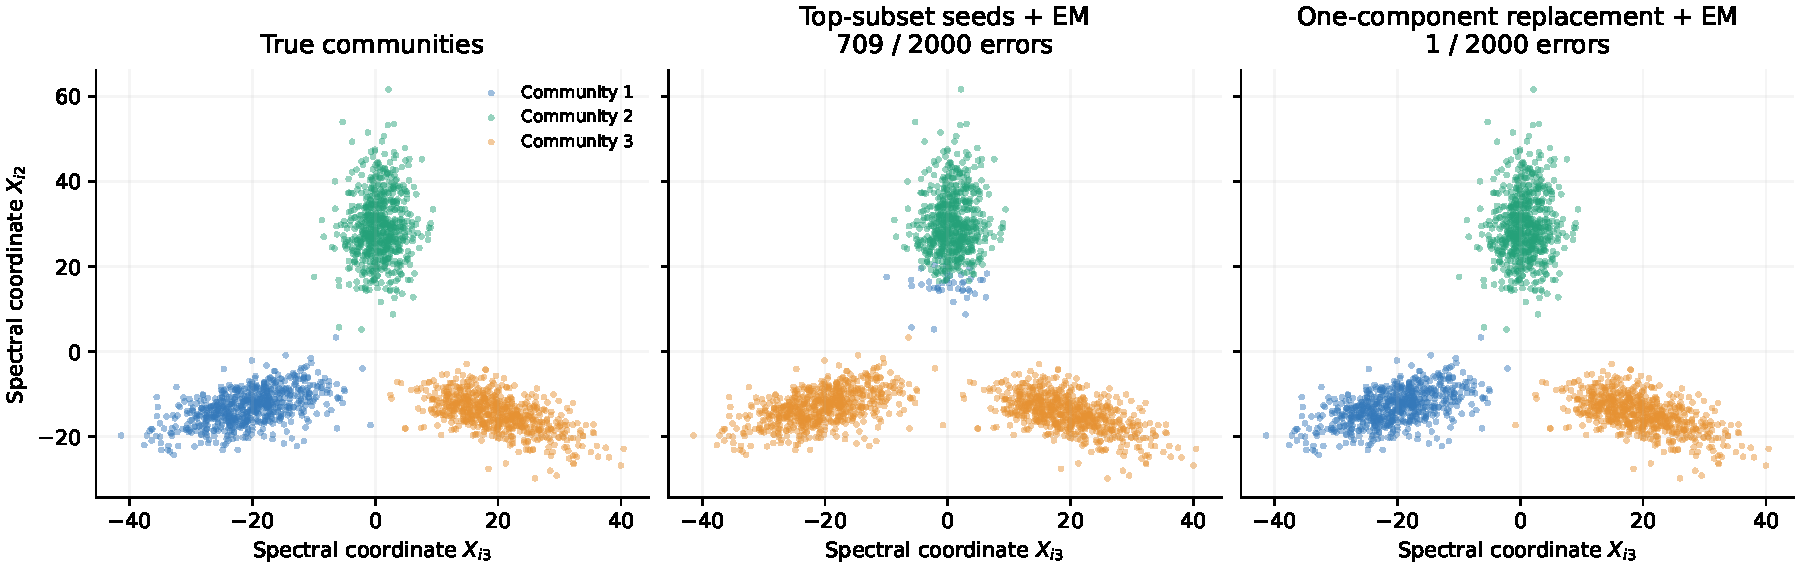
\includegraphics[width=\linewidth]{figures/initialization_failure_repair.pdf}
\caption{The saved design failure, displayed in two coordinates of
$X=\sqrt n U\Lambda$. Left: true communities, used only for evaluation.
Middle: top-subset peeling followed by EM merges the two lower communities
and splits the upper community. Right: an accepted one-component replacement
followed by EM separates the groups and leaves one mislabeled node. Predicted
labels are aligned to truth for display only.}
\label{fig:initialization_repair}
\end{figure}

\subsection{Historical numerical verification and computational scope}

All returned historical profile fits satisfy the declared stopping rule in the 240-graph
comparison. The 120 original peeling errors are reproduced exactly. The
archive contains 6240 EM traces, including replacement proposals, growing
stages, and restart fits, with 27867 recorded trace points. The smallest
observed objective increment is $-1.17\times10^{-10}$, within floating-point
rounding; no increment below $-10^{-7}$ occurs. All 240 selected ten-start
solutions maximize the same final working likelihood within their restart
set. Replacement accepts a likelihood improvement on 22 design graphs and
25 independent graphs, and never lowers the final objective; most of these
small improvements do not change the classification error. Independent
scalar checks reproduce deviance and global-gain calculations with maximum
absolute errors $7.11\times10^{-15}$ and $1.78\times10^{-15}$, respectively.

The present implementation explicitly reconstructs the $n\times n$ profiles
and caches all singleton-candidate scores. Reconstruction costs
$O(n^2K)$, score precomputation costs $O(n^3)$, and storage costs $O(n^2)$.
An EM update costs $O(n^2K)$. A replacement pass tries $K$ additional fits,
whereas ten-start residual seeding uses ten fits. The runs use one numerical
library thread per worker and four worker processes. Python, NumPy, SciPy,
and scikit-learn versions are 3.11.7, 2.1.3, 1.16.2, and 1.7.1. Stored timers
cover all candidate arms and restarts together and exclude graph generation
and eigenpair computation, so they do not support an arm-specific speed
claim. The data sizes $n\le2000$ establish feasibility for this implementation;
candidate-pool approximations and blockwise computations require separate
large-graph validation.

The archived comparisons support improved decoding of a fixed spectrum in
several heterogeneous models and identify a concrete failure of subset
initialization. The new 60-graph study directly evaluates the current
Algorithm~1 and records its weak-signal failures and its lack of a substantive
replacement improvement on that particular collection. Neither collection
estimates an asymptotic error exponent, proves uniform dominance over
$k$-means, or replaces the model assumptions and analysis of
Theorems~\ref{thm:main-recovery} and~\ref{thm:local-spectral-em}.

\paragraph{Companion sparse threshold-certificate checks.}
A separately retained sparse-score implementation tests a uniform-weight
refit together with the replacement trials and accepts only gains of at
least $(\sum_{ij}q_{ij})/\sqrt{\log n}$. Its archived checks contain 24
graphs with $n\in\{256,512\}$, $K\in\{3,4,6\}$, two degree scales,
and two seeds in one heterogeneous assortative family. They record 19 exact
recoveries and seven errors among 9,216 nodes; no natural growing endpoint
requires an accepted replacement in that collection. A separate injected
collapsed population endpoint is repaired in two accepted rounds. These
checks concern the companion sparse threshold rule, not the complete
Bernoulli Algorithm~1. They remain available as
\path{general_k_fresh_checks.json} beside that implementation.

% ---- conclusion ----
\section{Conclusion}
\label{sec:conclusion}

The retained adjacency eigenpairs can contain the likelihood information needed for nearly optimal community recovery. In a full-rank SBM, the population membership subspace contains the block-constant Bernoulli contrasts. First-order analysis of the empirical spectrum, clipping-aware exponential moments, and uniform parameter-fitting bounds make this relation quantitative for $p=\Omega(\log n/n)$ under the stated signal conditions. The complete nonedge term extends the score to dense graphs while preserving the weighted-mean M-step.

For every fixed $K$, repeated component replacement supplies the initialization guarantee. Its population contraction follows from matching $K$ true profiles to $K$ fitted profiles. Testing every deletion position and all observed candidates transfers that contraction to the fitted working objective. After $\lceil\log n\rceil$ rounds, low loss certifies weak responsibilities; the mandatory final update and likelihood classification give
\[
 \mathbb E\,\Mis(\widehat z,z)\le e^{-(1+o(1))I_n}.
\]
This is the leading oracle Chernoff exponent. The density condition makes expected degrees of order $np$; they may differ across communities and exceed logarithmic order. Neither $P/p$ nor the community proportions need converge. The comparability, probability ceiling and quantitative full-rank assumptions remain part of the result.

The proof concerns the complete algorithm with repeated replacement. General-$K$ recovery by the unchanged growing-only procedure remains open in the scope studied here. A certified population example rules out an unrestricted claim for one-update-per-stage growing. The new 60-graph benchmark verifies the revised implementation but shows no additional classification improvement from replacement and substantial errors in weak-signal models. These outcomes, together with the separately reported historical 240-graph results, motivate more extensive finite-sample study. Reducing the cubic candidate-cache cost and quadratic storage, relaxing the quantitative rank condition, and treating expected degrees below order $\log n$ are further questions.

\appendix
% ---- theory ----
\section{Probability bounds and local likelihood fitting}
\label{app:statistical-proofs}

Throughout the proofs, $p=\max_{a,b}P_{ab}$ is the probability scale in \eqref{eq:model-conditions}--\eqref{eq:density-condition}. The assumption $p=\Omega(\log n/n)$ ensures $\log n\le Cnp$ for a fixed constant $C$ and all sufficiently large $n$. All constants may depend on the fixed model bounds, the constant implicit in this density lower bound, $K$, and the admissible $c_0$, but not on the particular sequence of normalized matrices.

\subsection{Uniform information and the oracle leading exponent}
\label{app:uniform-density-bounds}

There are constants $c,C>0$ such that
\begin{equation}
 \min_{a\ne b}\|p_{a*}-p_{b*}\|_1\ge cnp,
 \qquad
 cnp\le D(p_{a*}\Vert p_{b*})\le Cnp,
 \qquad
 cnp\le D^*_{i,ab}\le Cnp.
 \label{eq:uniform-information-scale}
\end{equation}
To verify the lower bounds, note that
\[
 \|P_{a*}-P_{b*}\|_2
 =\|(e_a-e_b)^\top P\|_2
 \ge\sqrt2\,\kappa p.
\]
Positive community proportions transfer this bound to the full
profiles.  In particular their squared Euclidean separation is at
least $cnp^2$.  The scalar Bernoulli entropy has second
derivative $1/[x(1-x)]\ge1/p$ on the interval between two
true probabilities.  This proves the KL lower bound.  For Chernoff
information, use its value at $\alpha=1/2$ and
\[
 -\log\{\sqrt{uv}+\sqrt{(1-u)(1-v)}\}
 \ge\tfrac12(\sqrt u-\sqrt v)^2
 \ge\frac{(u-v)^2}{8p}.
\]
Omitting one coordinate changes the bound by $O(p)$.
For the upper bounds use $P_{ab}\ge\kappa p$ for every block pair and
$1-p\ge\eta$ in the usual Bernoulli KL upper bound.
Consequently $I_n\asymp np$.

\paragraph{The oracle leading exponent.}
The binary oracle Bayes risk obeys
$R^{\mathrm{or}}_{i,ab}=\exp\{-(1+o(1))D^*_{i,ab}\}$ uniformly.
For completeness, the upper bound is the exact Chernoff bound.
For the lower bound, tilt the product Bernoulli law by its
Chernoff-maximizing $\alpha$.  This maximizer is interior because
the two distributions differ and the endpoint divergences are zero.
The tilted mean of the oracle LLR is therefore zero.  The logit
contrasts are bounded uniformly under
\eqref{eq:model-conditions}--\eqref{eq:density-condition}, and each tilted Bernoulli
success probability is at most $Cp$, so the tilted LLR
variance is at most $Cnp$.  With $h=(np)^{2/3}$, Chebyshev's inequality
gives tilted probability $1-o(1)$ to $|L|\le h$.  On this event,
the two change-of-measure factors entering the binary Bayes risk
are both at least $e^{-D^*-h}$.  This proves the lower bound with
an $o(np)$ exponent loss.  Fixed nonzero prior odds add only $O(1)$
to the testing threshold.

\subsection{Exponential-confidence full-graph approximation}
\label{app:general-full-spectral}

\begin{proof}[Proof of Lemma~\ref{lem:full-spectral}]
The actual mean $M=\mathbb E[A\mid z]$ leaves
$\operatorname{col}(Z)$ invariant.  In its orthonormal membership
basis, the restriction of $M$ equals
\[
 (Z^\top Z)^{1/2}P(Z^\top Z)^{1/2}
       -\operatorname{diag}(P_{11},\ldots,P_{KK}).
\]
Its $K$ signal eigenvalues have absolute values between $cnp$ and
$Cnp$.  On the orthogonal complement, the eigenvalues are
$-P_{aa}$ and have magnitude at most $p$.
Let $U_*,\Lambda_*$ denote the signal eigenpairs.  Then
$U_*U_*^\top=\Pi_*$ and
$\|U_*\|_{2\to\infty}\le C/\sqrt n$.

We establish all probabilistic bounds at the scale $e^{-Hnp}$.
For the centered symmetric matrix $A-M$, its independent
upper-triangular entries have absolute value at most one and
maximum row variance sum at most $np$.  The centered-entry form of
Bandeira--van Handel's spectral norm bound
\citep[Corollary 3.12 and Remark 3.13]{bandeiravhandel2016} gives
\[
 \Pr\{\|A-M\|_{\mathrm{op}}>C\sqrt{np}+t\}
       \le n\exp(-t^2/C).
\]
Set $t=C_H\sqrt{np}$.  Since $\log n\le Cnp$, the constant can
be chosen so that
\begin{equation}
 \Pr\{\|A-M\|_{\mathrm{op}}>C_H\sqrt{np}\}
       \le e^{-Hnp}.
 \label{eq:exponential-spectral-norm}
\end{equation}
All confidence powers used within the proof may be increased to
absorb its finitely many union bounds.

We next verify the entrywise eigenspace bound, including its
confidence.  The Bernoulli row inequality of Abbe et al.
\citep[Lemma 7]{abbe2020} states that, for a fixed vector $w$,
independent Bernoulli $X_j$ with means at most the model bound $p$, and $\alpha\ge0$,
\[
 \Pr\left\{\left|\sum_jw_j(X_j-\mathbb EX_j)\right|
  >\frac{(2+\alpha)np\|w\|_\infty}
   {1\vee\log(\sqrt n\|w\|_\infty/\|w\|_2)}\right\}
       \le2e^{-\alpha np}.
\]
Choose a fixed $\alpha>H+2C$, where $C$ satisfies $\log n\le Cnp$.
Applying this bound to each of the at most
$K$ columns verifies their row-concentration assumption, with
total failure at most $e^{-Hnp}$ and with concentration function
\[
 \varphi_H(x)=\frac{C_H}{1\vee\log(1/x)},\quad x>0,
 \qquad \varphi_H(0)=0.
\]
For matrices, the column norms can be replaced by the Frobenius
and maximum row norms because $\varphi_H$ is nondecreasing and
$\varphi_H(x)/x$ is nonincreasing.  The fixed number of columns
only changes $C_H$.

The signal condition number is bounded.  Choose
$\gamma=C_H/\sqrt{np}$.  Their incoherence assumption follows from
$\|M\|_{2\to\infty}\le np/\sqrt n$ and $np\le n$;
their row/column independence assumption follows from independent
upper-triangular edges.  The norm assumption follows from
\eqref{eq:exponential-spectral-norm}.  Finally
$\gamma\to0$ and $\varphi_H(\gamma)\to0$, as required for the
smallness condition in their Theorem 2.1.

Apply that theorem to the positive and negative signal groups
separately.  Each is a contiguous eigenvalue group with a gap of
order $np$ to its complement.  Concatenating the polar alignments
gives an orthogonal $R$ and $V=UR$ such that
\begin{equation}
 \|V\|_{2\to\infty}\le C_H/\sqrt n,\qquad
 \|V-AU_*\Lambda_*^{-1}\|_{2\to\infty}
        \le\nu_{H,n}/\sqrt n,
 \label{eq:general-first-order}
\end{equation}
where $\nu_{H,n}\to0$.  Repeated eigenvalues inside a group do not
affect this argument.  The non-low-rank-mean form of the theorem
accounts for the absent diagonal.  The norm event also ensures
that the empirical eigenpairs with largest absolute eigenvalues
are precisely these signal groups.

Davis--Kahan with the same polar alignments gives
$\|V-U_*\|_{\mathrm{op}}\le C_H/\sqrt{np}$.
Put $T=R^\top\Lambda R=V^\top AV$.  Since
$\|M\|_{\mathrm{op}}=O(np)$,
\[
 \|T-\Lambda_*\|_{\mathrm{op}}
 \le\|A-M\|_{\mathrm{op}}
       +2\|M\|_{\mathrm{op}}\|V-U_*\|_{\mathrm{op}}
 \le C_H\sqrt{np}.
\]
A degree Chernoff bound, followed by a union bound and use of
$\log n\le Cnp$, also gives
$\max_i\deg(i)\le C_Hnp$ at the same confidence.  Hence
$\|(AU_*)_i\|_2\le C_Hnp/\sqrt n$.

Writing $E_1=V-AU_*\Lambda_*^{-1}$, the exact decomposition is
\[
 (U\Lambda U^\top-A\Pi_*)_i
 = (E_1)_iTV^\top
   +(AU_*)_i\{\Lambda_*^{-1}TV^\top-U_*^\top\}.
\]
The bracket has operator norm $O((np)^{-1/2})$.  Therefore
\[
 \|U\Lambda U^\top-A\Pi_*\|_{2\to\infty}
 \le C_H(np\nu_{H,n}+\sqrt{np})/\sqrt n
 =o(np/\sqrt n).
\]
Cauchy--Schwarz and the coordinatewise Lipschitz property of
clipping give the first bound in
\eqref{eq:general-profile-errors}.  This remains true when the
common clipping threshold is random.

The Perron eigenvalue of $M$ is between its minimum and maximum
row sums.  These sums lie in
$[(n-1)\kappa p,np]$.
The norm event consequently gives
$(\kappa/4)np\le s\le2np$ for all sufficiently large $n$.
Thus every true probability lies strictly between the clipping
endpoints.  The entrywise bound
\[
 |(U\Lambda U^\top)_{ij}|
 \le\|U_i\|_2\|\Lambda\|_{\mathrm{op}}\|U_j\|_2
 \le C_Hp
\]
then proves \eqref{eq:general-profile-box}.

For the remaining average bound, write
$N_{ic}=\sum_{j:z_j=c}A_{ij}$.  Projection onto the block-constant
space and contraction of clipping toward a true probability give
\[
 \|q_i^0-p_{z_i,*}\|_1
       \le\sum_c|N_{ic}-n_cP_{z_i,c}|.
\]
Let $F$ be the sum of the right-hand side over $i$.
Then $\mathbb EF\le Cn\sqrt{np}+Cnp$, where $Cnp$ includes the
missing-diagonal correction.  Changing one independent edge
changes $F$ by at most two.  The bounded-differences inequality
at deviation $n(np)^{3/4}$ yields
\[
 \Pr\{F-\mathbb EF>n(np)^{3/4}\}
       \le\exp(-c(np)^{3/2}).
\]
This is smaller than $e^{-Hnp}$ eventually for every fixed $H$.
Combine it with the uniform reconstruction error and enlarge a
deterministic $a_{H,n}\to0$ to finish the proof.
\end{proof}

\subsection{Clipping at a threshold estimated from the spectrum}
\label{app:general-clipped-chernoff}

Fix true class $a$ and competitor $b$, and write
\[
 w_c=\log\frac{P_{ac}(1-P_{bc})}{P_{bc}(1-P_{ac})},
 \qquad b_c=\log\frac{1-P_{ac}}{1-P_{bc}},
 \qquad
 N'_{ic}=n_c\operatorname{clip}
       (N_{ic}/n_c,\varepsilon_n,1-\varepsilon_n).
\]
The true-profile working contrast based on $q_i^0$ is
\begin{equation}
 L_{i,\mathrm{clip}}^{ab}
       =\sum_c N'_{ic}w_c+\sum_c n_cb_c.
 \label{eq:general-clipped-score}
\end{equation}
For every deterministic $t_n=o(np)$, it satisfies
\begin{equation}
 \Pr_a\{G_H,\ L_{i,\mathrm{clip}}^{ab}\le t_n\}
       \le2^K\exp\{-D^*_{i,ab}+o(np)\}.
 \label{eq:general-clipped-chernoff}
\end{equation}
The event $G_H$ is from
Lemma~\ref{lem:full-spectral}.  We prove the statement
without conditioning on the random clipping threshold.

Put $\varepsilon_+=2c_0p$.  On $G_H$,
$\varepsilon_n\le\varepsilon_+$; and for all sufficiently large
$n$ every binomial mean $\mathbb E_aN_{ic}$ lies inside
$[n_c\varepsilon_+,n_c(1-\varepsilon_+)]$, including the omitted
self-loop.  If $w_c<0$, then on $G_H$,
\[
 N'_{ic}\le\max\{N_{ic},n_c\varepsilon_+\}.
\]
If $w_c\ge0$, then on $G_H$,
\[
 N'_{ic}\ge\min\{N_{ic},n_c(1-\varepsilon_+)\}.
\]
These are deterministic-threshold bounds in the direction that
upper-bounds $\exp(-\alpha w_cN'_{ic})$ for $\alpha\in[0,1]$.

For $\beta\ge0$ and $u\le\mathbb EN$,
\[
 \mathbb Ee^{\beta\max(N,u)}
 \le\mathbb Ee^{\beta N}+e^{\beta u}
 \le2\mathbb Ee^{\beta N}.
\]
For $\beta\le0$ and $v\ge\mathbb EN$, the analogous inequality is
\[
 \mathbb Ee^{\beta\min(N,v)}
 \le\mathbb Ee^{\beta N}+e^{\beta v}
 \le2\mathbb Ee^{\beta N}.
\]
The second step in each line is Jensen's inequality.  The
deterministic envelopes depend on independent block counts, so
their exponential moments factor.  Hence
\begin{equation}
 \mathbb E_a\left[\mathbf1_{G_H}
        e^{-\alpha L_{i,\mathrm{clip}}^{ab}}\right]
 \le2^K\exp\{-D_\alpha(p_{a,-i}\Vert p_{b,-i})+O(p)\}.
 \label{eq:general-clipped-moment}
\end{equation}
The only offset discrepancy between the raw working contrast and
the oracle LLR is $b_{z_i}$ from retaining the reconstructed
diagonal.  It is $O(p)$, and in particular is $o(np)$.
Exponential Markov inequality at a maximizing $\alpha$ proves
\eqref{eq:general-clipped-chernoff}.  No independence of
$\varepsilon_n$ and the incident edges has been asserted.

\subsection{Deterministic fitting bounds and an invariant basin}
\label{app:general-local-em}

On $G_H$, all observed profiles and their convex combinations
belong to the box
\begin{equation}
 cp\le x_j\le
          \min\{C_Hp,1-cp\}.
 \label{eq:general-common-box}
\end{equation}
True profiles also lie in this box after adjusting its constants.
Ratios $x_j/y_j$ are uniformly bounded.  The same is true of
$(1-x_j)/(1-y_j)$: if $C_Hp\le1/2$, both complements
are at least $1/2$; otherwise they are at least
$c/(2C_H)$.  As a consequence, on this box,
\begin{align}
 0\le D(x\Vert y)&\le C_Hnp,\\
 |D(x\Vert y)-D(x'\Vert y')|
   &\le C_H(\|x-x'\|_1+\|y-y'\|_1),
 \label{eq:general-deviance-lipschitz}\\
 D(x\Vert y)&\ge
                 \frac{\|x-y\|_1^2}{2C_Hnp}.
 \label{eq:general-deviance-coercive}
\end{align}
The Lipschitz claim follows by differentiating the scalar
divergence; its two derivatives are
$\operatorname{logit}(x)-\operatorname{logit}(y)$ and
$(y-x)/[y(1-y)]$.  The lower bound follows from
$[x(1-x)]^{-1}\ge(C_Hp)^{-1}$ and Cauchy--Schwarz.
The derivative of the fitting score with respect to a parameter
coordinate $y$ is $(q-y)/[y(1-y)]$, which is also uniformly bounded
on the common box.

\begin{proof}[Proof of Theorem~\ref{thm:local-spectral-em}]
Fix $H>1+\limsup I_n/(np)$, finite by \eqref{eq:uniform-information-scale}. Suppose $R$ is a responsibility matrix whose aligned average
error is at most $\gamma$, below a sufficiently small fixed
constant.  Write $N_a=\sum_iR_{ia}$ and
$\bar q_a=n_a^{-1}\sum_{i:z_i=a}q_i$.  The average profile bound
gives $\|\bar q_a-p_{a*}\|_1\le C_Ha_{H,n}np$.
Moreover $|N_a-n_a|\le n\gamma$ and
$N_a\ge\pi_0n/2$.  The exact M-step identity implies
\[
 \|\widehat p_a-\bar q_a\|_1
 \le\frac{\sum_i|R_{ia}-Z_{ia}|\|q_i\|_1}{N_a}
    +\left|\frac{n_a}{N_a}-1\right|\|\bar q_a\|_1
 \le C_H\gamma np.
\]
Consequently
\begin{equation}
 \max_a\|\widehat p_a-p_{a*}\|_1
       \le C_H(\gamma+a_{H,n})np.
 \label{eq:general-local-profile-fit}
\end{equation}
The updated weights have bounded log-ratios: this follows from
$N_a/n\ge\pi_0/2$ for the unconstrained update, or from a fixed
positive floor for the exact floored-simplex optimizer.

Define $\widehat\ell_i(a)=\ell_i(\widehat p_a)+\log\widehat\pi_a$. Using the score derivatives just established and the uniform
$q-q^0$ bound, every fitted contrast therefore satisfies
\begin{equation}
 \left|\widehat\ell_i(a)-\widehat\ell_i(b)
       -L_{i,\mathrm{clip}}^{ab}\right|
       \le C_H(\gamma+a_{H,n})np+C_H.
 \label{eq:general-local-score-fit}
\end{equation}
This is a deterministic bound on $G_H$, uniform over all such
responsibilities.  It requires no independence among the fit,
the spectrum, and the incident edges.  If $\gamma=\gamma_n\to0$,
a wrong label implies
$L_{i,\mathrm{clip}}^{ab}\le o(np)$ for some competitor, apart
from the graph and initialization failures.  Equation
\eqref{eq:general-clipped-chernoff} therefore proves the
one-update leading exponent.

To handle all later exact updates, use the uniform true-profile
margin $D(p_{a*}\Vert p_{b*})\ge cnp$ from
\eqref{eq:uniform-information-scale}.  Choose a sufficiently
small fixed responsibility radius $\gamma_0$ and row tolerance
$t_0>0$.  Equations \eqref{eq:general-local-profile-fit} and
\eqref{eq:general-deviance-lipschitz} then imply a correct-class
margin of at least $c'np$ whenever $\gamma\le\gamma_0$ and
$\|q_i-p_{z_i,*}\|_1\le t_0np$.  At most $a_{H,n}/t_0$ of the
rows violate the latter condition.  The next E-step hence has
aligned average responsibility error at most
\begin{equation}
 b_{H,n}=2a_{H,n}/t_0+2(K-1)e^{-c'np}\longrightarrow0.
 \label{eq:general-basin-invariance}
\end{equation}
For large $n$, this is below $\gamma_0$.  Starting at error
$\gamma_n\to0$, every later responsibility matrix consequently
has error at most $\max\{\gamma_n,b_{H,n}\}=o(1)$ on the same
event.  The score bound has one deterministic $o(np)$ remainder
for all later iterations.  This covers any finite, possibly
data-dependent stopping time after the first M-step without
an iteration union bound.

If the weak-initialization failure probability $\delta_n$
satisfies
$\liminf(-\log\delta_n)/I_n\ge1$, choose
$H>1+\limsup I_n/(np)$, which is finite by
\eqref{eq:uniform-information-scale}.  Summing the pairwise
clipped bounds and adding the exceptional probabilities gives
\[
 \mathbb E\operatorname{Mis}(\widehat z,z)
 \le\delta_n+C_He^{-Hnp}
       +(K-1)2^K\exp\{-I_n+o(np)\}
 \le\exp\{-(1+o(1))I_n\}.
\]
For a deterministic initialization or replacement proof valid
on $G_H$, the only exceptional probability is the graph failure,
so there is no additional random-start confidence requirement.
Finally $\liminf I_n/\log n>1$ implies exact recovery by
Markov's inequality applied to the number of mislabeled nodes.
\end{proof}


\section{Deterministic initialization by likelihood replacement}
\label{app:replacement-proof}

\subsection{Exact EM and the profile constraint}
For any nonnegative responsibilities with rows summing to one, define
\[
 \mathcal Q(R,\widehat\pi,\widehat p)
 =\sum_{i,a}R_{ia}\{\log\widehat\pi_a+\ell_i(\widehat p_a)-\log R_{ia}\}.
\]
The log-sum inequality gives $\mathcal Q\le\mathcal L$, with equality at the E-step. For fixed $R$, the profile-coordinate objective is
\[
 \left(\sum_iR_{ia}q_{ij}\right)\log\widehat p_{aj}
 +\left(N_a-\sum_iR_{ia}q_{ij}\right)\log(1-\widehat p_{aj}).
\]
Its maximizer for $N_a>0$ is the weighted mean in \eqref{eq:mstep}; maximizing $\sum_aN_a\log\widehat\pi_a$ over the simplex gives $\widehat\pi_a=N_a/n$. Thus every exact E/M pair raises $\mathcal L$ and lowers $F$. A zero-mass component contributes nothing to this objective and may retain its previous profile. All nonzero-mass updates are convex combinations of the $q$ rows. These observations also prove that all means remain in the common box on $G_H$.

Since $D(q_i\Vert\widehat p_a)\ge0$, the objective is bounded above by the observation-only saturated score $S_q$. Consequently an infinite exact EM sequence has convergent objective values. This fact alone gives neither a global optimum nor community recovery. The replacement argument below supplies the latter conclusion from a different, finite-round bound.

\subsection{Empirical replacement and soft-loss contraction}
\begin{proof}[Proof of Theorem~\ref{thm:replacement-contraction}]
In this proof use its deterministic common-box assumption and write $\beta=1-1/K$. The Bernoulli divergence derivatives are
\[
 \partial_xD(x\Vert y)=\log\frac{x(1-y)}{y(1-x)},\qquad
 \partial_yD(x\Vert y)=\frac{y-x}{y(1-y)}
\]
for one coordinate. The box makes both derivatives uniformly bounded by a constant $L$. The multivariate divergence therefore satisfies
\[
 |D(x\Vert y)-D(x'\Vert y')|
 \le L(\|x-x'\|_1+\|y-y'\|_1).
\]
For any admissible center list $\mathcal C$, define the population loss using the same $n_a$ as in the sample. Taking minima is Lipschitz under a uniform coordinatewise perturbation, so
\begin{equation}
 \sup_{\mathcal C}|G(\mathcal C)-G_*(\mathcal C)|
   \le L\sum_i\|q_i-p_{z_i,*}\|_1
   \le La_n n^2p.
 \label{eq:uniform-hard-loss}
\end{equation}
This statement is simultaneous over center lists; their dependence on the data and all previous fits is immaterial.

Every true class contains a node $c_a$ with
\begin{equation}
 \|q_{c_a}-p_{a*}\|_1\le a_n np/\pi_0.
 \label{eq:available-good-candidate}
\end{equation}
Indeed, the total deviation within that class is at most $a_n n^2p$, while its size is at least $\pi_0n$. Apply Lemma~\ref{lem:population-replacement} to the current list to find $a,r$. Replacing its ideal new profile $p_{a*}$ by this observed $q_{c_a}$ changes each available minimum loss by at most $L\|q_{c_a}-p_{a*}\|_1$. Applying \eqref{eq:uniform-hard-loss} before and after the population replacement yields
\begin{align*}
 G(\mathcal C^{r\leftarrow q_{c_a}})
 &\le G_*(\mathcal C^{r\leftarrow p_{a*}})
             +La_n n^2p+La_n n^2p/\pi_0\\
 &\le\beta G_*(\mathcal C)+La_n n^2p+La_n n^2p/\pi_0\\
 &\le\beta G(\mathcal C)+Ba_n n^2p
\end{align*}
for a fixed constant $B$.

The executable gain finds a candidate at least this good. For any deletion $r$ and candidate $c$, saturation gives the exact identity
\begin{equation}
 G(\mathcal C^{r\leftarrow q_c})
  =G(\mathcal C\setminus\{\mu_r\})
     -\sum_i\bigl(\ell_i(q_c)-h_i^{(-r)}\bigr)_+.
 \label{eq:gain-hard-loss-identity}
\end{equation}
Thus the maximizing node in \eqref{eq:replacement-gain} minimizes hard loss for that deletion. All $K$ deletions are tested, so at least one of the actual trials has initial hard loss at most $\beta G(\mathcal C)+Ba_n n^2p$.

Initialize that trial's weights uniformly. The log-sum bound in \eqref{eq:soft-hard} gives initial soft loss at most $\beta G(\mathcal C)+Ba_n n^2p+n\log K$. Any subsequent exact EM fit only decreases this loss. Selection among the trial endpoints and the old fit therefore gives
\[
 F_{t+1}\le\beta G(\mathcal C_t)+Ba_n n^2p+n\log K
          \le\beta F_t+Ba_n n^2p+n\log K.
\]
Also $F_{t+1}\le F_t$ because the old fit is included.

On the box, every $D(q_i\Vert\mu_k)\le Mnp$ for a fixed $M$. For any simplex weights,
$\sum_k\widehat\pi_ke^{-D(q_i\Vert\mu_k)}\ge e^{-Mnp}$,
so $0\le F_0\le Mn^2p$ even when some weights vanish. Iterating the contraction gives
\[
 \frac{F_{T_n}}{n^2p}
 \le M\beta^{T_n}+KB a_n+\frac{K\log K}{np}.
\]
Fixed $K$, $T_n=\lceil\log n\rceil\to\infty$, and $np\to\infty$ make this bound vanish. This proves both displayed claims.
\end{proof}

Early termination after a round with no improving trial is also valid. In that round $F_{t+1}=F_t$, so the contraction itself gives
\[
 F_t\le K\{Ba_n n^2p+n\log K\}=o(n^2p).
\]
Thus a failed full replacement round is a weak-loss certificate even if later trial iteration budgets would differ. Under the fixed trial protocol used in the implementation, repeating unchanged deterministic trials also gives the same result. More generally, keeping a fit within a fixed $\zeta>0$ of the best trial adds $\zeta$ to the contraction remainder and $K\zeta/(n^2p)=o(1)$ to the final normalized bound. This observation does not assert an arbitrary floating-point error guarantee.

\subsection{Low loss certifies all \texorpdfstring{$K$}{K} communities}
\begin{proof}[Proof of Lemma~\ref{lem:low-loss-responsibilities}]
Work on $G_H$ and write $a_n=a_{H,n}$. There are deterministic $\xi_n\to0$ with $F\le\xi_n n^2p$ for the fits under consideration. The Bernoulli entropy curvature on the common box gives
\[
 D(x\Vert y)\ge\frac{\|x-y\|_1^2}{2C_Hnp}.
\]
Since $G\le F$,
\[
 \sum_i\min_k\|q_i-\mu_k\|_1^2\le2C_H\xi_n n^3p^2.
\]
Set $u_n=\sqrt{a_n}+\xi_n^{1/4}+(np)^{-1}\to0$. The fractions of rows farther than $u_n np$ from their true profile or farther than $u_n np$ from every fitted profile are at most $a_n/u_n$ and $2C_H\xi_n/u_n^2$, respectively. Both vanish. Each true community of size at least $\pi_0n$ has a row outside these two exceptional sets. Its true profile therefore lies within $2u_n np$ of some fitted profile.

Equation~\eqref{eq:uniform-information-scale} separates distinct true profiles by at least a fixed positive multiple of $np$. For all sufficiently large $n$, different true profiles must therefore match different fitted profiles. There are exactly $K$ of each, giving one common permutation with
\begin{equation}
 \max_a\|\mu_a-p_{a*}\|_1\le2u_n np.
 \label{eq:matched-profiles}
\end{equation}
Write the true-profile separation constant as $s_0>0$. On a row with $\|q_i-p_{z_i,*}\|_1\le u_n np$, every wrongly matched fitted profile is at least $s_0np/2$ away in $\ell_1$ norm, and its divergence is at least $c_1np$ for $c_1=s_0^2/(8C_H)>0$.

For the selected fit's exact E-step, the identity \eqref{eq:variational-loss} remains valid with zero weights using zero-responsibility conventions. Summing that identity over typical rows bounds total wrong responsibility by $F/(c_1np)$. Each other row contributes at most two to the $\ell_1$ error. Consequently
\[
 \frac1n\sum_{i,a}|R_{ia}-Z_{ia}|
 \le\frac{2a_n}{u_n}+\frac{2\xi_n}{c_1}\longrightarrow0.
\]
The bound is deterministic and uniform over the indicated class of fits on $G_H$.
\end{proof}

\subsection{Completion of the algorithmic guarantee}
\begin{proof}[Proof of Theorem~\ref{thm:main-recovery}]
Choose a fixed $H>1+\limsup_n I_n/(np)$, which is possible by \eqref{eq:uniform-information-scale}. On $G_H$, all $q$ rows, the global mean, and every mean generated by growing or replacement lie in the same common box. Thus Theorem~\ref{thm:replacement-contraction} applies to the growing endpoint irrespective of its labels or mixture weights. Its $T_n$ rounds give $F\le\xi_n n^2p$ for a deterministic $\xi_n\to0$.

Lemma~\ref{lem:low-loss-responsibilities} certifies the selected fit's responsibilities with a deterministic error $\gamma_n\to0$ on $G_H$. The probability of failure is at most $C_He^{-Hnp}$, which is negligible at the $e^{-I_n}$ scale. The final profile and weight M-step in Algorithm~1 therefore invokes Theorem~\ref{thm:local-spectral-em} and gives \eqref{eq:main-rate}. That theorem also covers any additional finite exact updates.

Finally $n\Mis$ is an integer, so
$\Pr\{\Mis>0\}\le n\E\Mis$.
When $\liminf I_n/\log n>1$, the right side tends to zero. The stated dense candidate computations, $O(\log n)$ replacement rounds and finite polynomial fitting caps establish polynomial running time. This proof includes initialization and parameter fitting and has no random-restart failure event.
\end{proof}

\subsection{Sparse-score comparison}
For completeness, when $p\to0$, the exact Bernoulli contrast can be written as
\[
 \sum_{j\ne i}A_{ij}\log\frac{p_{aj}}{p_{bj}}
 +\sum_{j\ne i}A_{ij}\log\frac{1-p_{bj}}{1-p_{aj}}
 +\sum_{j\ne i}\log\frac{1-p_{aj}}{1-p_{bj}}.
\]
For $u,v\le p\le1/2$, Taylor's formula gives
$|\log(1-u)+u|\le Cu^2$ and
$|\log(1-u)-\log(1-v)|\le C p$.
Subtracting the sparse contrast therefore leaves at most
$C\{p\deg(i)+np^2\}$ in absolute value. A degree Chernoff bound at any prescribed confidence $e^{-Hnp}$ makes this $O(np^2)=o(np)$. There is no need to require $np^2=o(1)$. The dense example in the main text follows from the Bernoulli large-deviation exponent at the two stated thresholds and shows why dropping the nonedge term is not generally allowed when $p$ is bounded below.

% ---- implementation ----
\section{Implementation and reproducibility}
\label{app:implementation}

\subsection{Current implementation}
The source, complete numerical evidence and compiled manuscript are at
\begin{center}
\url{https://github.com/zhixin0825/spectral-lrt}.
\end{center}
Algorithm~1 is implemented by \texttt{SpectralLikelihood.decode()} in
\begin{center}
\small\path{experiments/20261010_general_density/spectral_likelihood.py}.
\end{center}
It accepts an $n\times K$ eigenvector array and a length-$K$ array of the corresponding signed eigenvalues. The decoder receives neither the adjacency matrix, true labels, true block probabilities nor node degrees. Retaining the top-$|\lambda|$ eigenpairs is the preceding spectral step.

The default \texttt{score\_family='bernoulli'} evaluates \eqref{eq:working-score}. The floor coefficient defaults to $c_0=10^{-4}$; its theoretical guarantee requires the explicit admissibility condition in Section~\ref{sec:algorithm}, not merely positive block probabilities. The spectral scale is $\max\{1,\max_a|\lambda_a|\}$, and the reconstructed entries are clipped on both sides. The original adjacency is not regularized. The optional \texttt{score\_family='sparse'} is a score control on precisely the same $q$, and is not the default general-density algorithm.

Growing uses at most 100 exact M-steps per stage. A fit stops after at least one M-step if hard labels are unchanged and its absolute soft-loss change is at most $10^{-9}n$. Replacement uses at most $\lceil\log n\rceil$ rounds, tries every component deletion against the same incumbent, initializes each trial's weights uniformly, and uses one M-step per trial by default. A full round with no improvement stops the search. This rule is justified by the contraction certificate in Appendix~\ref{app:replacement-proof}. Calling \texttt{decode()} always executes the final E-step and one profile/weight M-step before returning labels.

The implementation uses the unconstrained simplex weight update. Zero-mass components retain their previous profile. Log-sum-exp arithmetic evaluates responsibilities and the soft divergence loss $F$ without exponentiating very negative raw log-likelihoods. Theoretical divergences are nonnegative; the code clips negative floating-point residue at zero. Weighted means, including the initial global mean, are clipped back to the same feasible interval solely to correct roundoff in convex combinations. The theorem is an exact-arithmetic result; recorded numerical checks assess implementation accuracy to floating-point precision.

The user may increase either fitting budget. Explicitly requesting fewer replacement rounds is an experimental option and does not automatically retain the stated general-$K$ initialization guarantee. The proven default budget is $\lceil\log n\rceil$, with valid early stopping after a full unsuccessful round.

\subsection{Current finite-graph and population evidence}
The complete 60-graph design is specified by
\begin{center}
\small\path{experiments/20261010_general_density/benchmark_results/protocol.json}.
\end{center}
It fixes all graph seeds, model families, density settings, method parameters, and hashes of the code used at fitting time. Each graph directory retains the original $A$, $P$, true labels for evaluation, exact retained $(U,\Lambda)$, all fitted profiles and weights, every candidate's hard loss, and full EM objective traces. Ground truth is not used for fitting, selecting replacements, or stopping. The aggregate CSV contains all 360 graph--method combinations.

The archived fitting engine is retained as \texttt{engine\_at\_fitting.py}. A subsequent boundary fix clips the rounded initial mean when a graph has all reconstructed entries at the floor. The maintenance record checks that this expression is bitwise unchanged on every archived graph, so the saved benchmark is unaffected. The original fitting hashes remain in the frozen protocol; maintenance provenance is recorded separately.

The five-community population calculation and the exact rational interval certificate are in
\begin{center}
\small\path{experiments/20261010_general_density/population_audit/}.
\end{center}
They record the positive-definiteness certificate, strict all-node-gain comparisons, the limiting one-update-per-stage trajectory, and replacement trial results. The distinction between a population limiting path, a finite-graph theorem, and fully iterated growing is maintained in the report. The manifest \texttt{SHA256SUMS} identifies the saved numerical records.

\subsection{Historical experiments and entry points}
The earlier 240-graph comparison is preserved at
\path{experiments/20261009_residual_likelihood_seeding/}.
The \texttt{residual\_seed.py} module retains several sparse-score methods, using
\[
 \ell_i^{\mathrm{sparse}}(\widehat p)=\sum_jq_{ij}\log\widehat p_j-\sum_j\widehat p_j.
\]
Its current default \path{method='global_gain_certified'} calls the separate sparse threshold-certificate implementation \texttt{Work.iterative\_certified\_growing()}. It uses an adaptive lower-only floor, a uniform-weight refit of the current centers as well as $K$ replacement trials, acceptance threshold $(\sum_{ij}q_{ij})/\sqrt{\log n}$, and a cap of $\lceil(\log n)^2\rceil$ accepted rounds. Its general-$K$ proof for the sparse range $p\to0$ with $p=\Omega(\log n/n)$ and its 24-graph implementation checks are retained as a companion version. They preceded the complete Bernoulli density extension and direct soft-loss contraction presented here, which allow the full range \eqref{eq:density-condition}.

In that module, \path{method='global_gain'} is the growing-only branch, \path{method='global_gain_restarts'} selects independent residual starts, and \path{method='repair'} is the historical single-pass repair. None identifies the current full-Bernoulli Algorithm~1, whose entry point is specified above. The actual 240-graph runs used the earlier lower floor $10^{-4}\log n/n$ and their recorded protocol, not the adaptive-floor default now present in the companion module. Their profiles were not constrained to lie below one. The preserved benchmark runner explicitly selects \texttt{floor\_mode='historical'} for these original arms; their earlier source is also accessible in repository history.

The archived 240-graph fits use an exact weight M-step with floor $f=10^{-8}$. For a fixed $0\le f<1/K$, it solves
\[
 \max_{\pi_a\ge f,\,\sum_a\pi_a=1}\sum_aN_a\log\pi_a,
 \qquad \pi_a=\max\{f,N_a/\lambda\},
 \quad\sum_a\pi_a=1.
\]
An active-set solver determines $\lambda$; naive clipping and renormalization is not this optimizer. The current main theorem and implementation use $f=0$.

Historical fits stop only when labels are unchanged, relative profile and absolute weight changes are at most $10^{-3}$, and the objective increment is at most $10^{-6}(1+|\mathcal L-G|)$, where $G=\sum_{ij}\log\Gamma(q_{ij}+1)$ is an observation-only tolerance constant. The cap is 300 updates. Historical top-subset and peeling controls, their subset sizes and stopping rules are defined by the archived code. They are not steps of Algorithm~1.

\subsection{Build and validation}
The active manuscript contains five main sections, statistical and deterministic proof appendices, implementation details, and references. PDFLaTeX, BibTeX and two further PDFLaTeX passes resolve the bibliography and cross references. Build provenance records the source revision and source/PDF checksums. The manuscript is rendered for a page-by-page layout check. These syntax, reference and layout checks are separate from the mathematical audit and numerical evidence described above.

\bibliographystyle{plainnat}
\bibliography{reference}
\end{document}
